%%% Local Variables:
%%% mode: latex
%%% TeX-master: t
%%% End:

\documentclass[bachelor]{thuthesis}
%\documentclass[master]{thuthesis}
%\documentclass[doctor]{thuthesis}
% \documentclass[%
%   bachelor|master|doctor|postdoctor, % mandatory option
%   secret,
%   openany|openright,
%   arialtoc,arialtitle]{thuthesis}

% 所有其它可能用到的包都统一放到这里了,可以根据自己的实际添加或者删除。
\usepackage{thutils}
\usepackage{listings}
\usepackage{pdfpages}
\usepackage{graphicx}

% 你可以在这里修改配置文件中的定义,导言区可以使用中文。
% \def\myname{薛瑞尼}

\begin{document}

% 定义所有的eps文件在 figures 子目录下
\graphicspath{{figures/}}


%%% 封面部分
\frontmatter

%%% Local Variables:
%%% mode: latex
%%% TeX-master: t
%%% End:
\secretlevel{公开} \secretyear{2100}

\ctitle{基于AS编址的互联网可扩展路由机制的仿真评价与测试}
% 根据自己的情况选,不用这样复杂
\makeatletter
\ifthu@bachelor\relax\else
  \ifthu@doctor
    \cdegree{工学博士}
  \else
    \ifthu@master
      \cdegree{工学硕士}
    \fi
  \fi
\fi
\makeatother


\cdepartment[计算机]{计算机科学与技术系}
\cmajor{计算机科学与技术}
\cauthor{王庆}
\csupervisor{王之梁副研究员}
% 如果没有副指导老师或者联合指导老师,把下面两行相应的删除即可。
%\cassosupervisor{施新刚副教授}
% \ccosupervisor{某某某教授}
% 日期自动生成,如果你要自己写就改这个cdate
%\cdate{\CJKdigits{\the\year}年\CJKnumber{\the\month}月}

% 博士后部分
% \cfirstdiscipline{计算机科学与技术}
% \cseconddiscipline{系统结构}
% \postdoctordate{2009年7月——2011年7月}

\etitle{Bandwidth Guarantee for Tenant Networks in Datacenter Clouds}
% 这块比较复杂,需要分情况讨论:
% 1. 学术型硕士
%    \edegree:必须为Master of Arts或Master of Science(注意大小写)
%              “哲学、文学、历史学、法学、教育学、艺术学门类,公共管理学科
%               填写Master of Arts,其它填写Master of Science”
%    \emajor:“获得一级学科授权的学科填写一级学科名称,其它填写二级学科名称”
% 2. 专业型硕士
%    \edegree:“填写专业学位英文名称全称”
%    \emajor:“工程硕士填写工程领域,其它专业学位不填写此项”
% 3. 学术型博士
%    \edegree:Doctor of Philosophy(注意大小写)
%    \emajor:“获得一级学科授权的学科填写一级学科名称,其它填写二级学科名称”
% 4. 专业型博士
%    \edegree:“填写专业学位英文名称全称”
%    \emajor:不填写此项
\edegree{Master of Science}
\emajor{Computer Science and Technology}
\eauthor{Wang Jingyi}
\esupervisor{Professor Yin Xia}
%\eassosupervisor{Shi Xingang}
% 这个日期也会自动生成,你要改么?
% \edate{December, 2005}

% 定义中英文摘要和关键字
\begin{cabstract}
  互联网的不断完善和扩展,网络设备和终端设备数量的不断增加,IPv4地址处于枯竭的状态,从IPv4过渡到IPv6的技术逐渐成熟,IPv6 地址本身的诸多优势,都预示未来IPv6网络将会迅速发展,由此带来的IPv6网络路由的可扩展性、收敛性和安全性问题值得研究。

  本文为了解决IPv6网络带来的可扩展路由问题,对已有的基于无类AS编址的CABA(Classless AS Based Addressing)方案以及基于自治系统号的域间路由机制A-BGP(ASN based BGP) 进行仿真评价与测试,验证其对路由可扩展性的作用。该CABA编址方案将自治系统号嵌入到IPv6 的地址中,兼容现有的IPv6 方案,可以实现增量部署。该A-BGP近需向外宣告一条嵌入自治系统号的前缀,这将极大程度的减少全局路由表的大小,同时也会减少UPDATE包的数目以及路由震荡的频率和收敛时间,尽可能解决IPv6 网络带来的可扩展路由问题。

  本文主要进行了以下工作;

  \begin{enumerate}
  \item 通过仿真和测试评价,在新型的无类AS的IPv6编址方案下基于自治系统号的域间路由机制A-BGP(ASN based BGP),对路由可扩展性的影响。
  \item 通过评估基于互联网路由表的FIB表压缩情况验证A-BGP对路由可扩展性的作用。结果显示A-BGP下的FIB表项是现网络中FIB表的10\%。
  \item 通过SIMBGP仿真在全网拓扑结构下宣告UPDATE的数目验证A-BGP对路由可扩展性的作用。分析SIMBGP中向外广播嵌入自治系统号的IPv6 前缀和广播现在网络中已宣告的IPv4的update包数,结果显示当前网络自治系统广播出去的prefix 越多,采用新型A-BGP机制发出的update数目越少。
  \item 通过测试小型拓扑结构下BGP路由表表项的数目验证A-BGP对路由可扩展性的作用。其中使用Docker软件运行多台Quagga软件路由器,部署自治系统均为Tier1层级的小型拓扑,向外宣告路由,结果显示其全局BGP路由表项从现有的9000多条减少到17条。
  \end{enumerate}
\end{cabstract}

\ckeywords{自治系统, 域间路由, 可扩展路由}

\begin{eabstract}
With Internet improving and expanding and the number of network terminal equipments increasing, IPv4 address is exhausted. The technical from IPv4 to IPv6 is mature and there are many advantages in IPv6, so IPv6 network will develop rapidly in the future, which may result in some problems, including IPv6 network routing scalability, convergence and security issues and so on.

In this thesis, we do some simulations and tests to verify the IPv6 network routing scalability under the new IPv6 addressing scheme based AS, called CABA (Classless AS Based Addressing) and the new inter-domain routing mechanism called A-BGP (ASN based BGP). This scheme is compatible with existing addressing scheme, and the autonomous system only needs to broadcast one prefix, which embedded the autonomous system number. This could not only greatly reduce the size of the global routing table, but also reduce the number of BGP update packets and routing flapping frequency and convergence time.

This thesis mainly for the following work;


\begin{enumerate}
\item Explain the new IPv6 addressing scheme called CABA and the new inter-domain routing mechanism called A-BGP.
\item Compare the number of current FIB table and the number of new FIB table based CABA and A-BGP to verify the IPv6 network routing scalability. The result shows the new FIB table is 10\% of the current.
\item Conduct simulations by SIMBGP on the CABA and A-BGP to verify IPv6 network routing scalability. The result shows that autonomous system of announcing more prefixs can reduce more UPDATE packets under new mechanism.
\item Realize a virtual network environment based the CABA and A-BGP to verify the IPv6 network routing scalability. Use Docker to realize virtual software router, check the number of BGP routing table in the topology of Tier 1.The result shows BGP routing tables reduce from about 9000 to 17 in the new mechanism A-BGP.
\end{enumerate}

\end{eabstract}

\ekeywords{Autonomous System, Inter-domain, Scalable Routing}

% 设置 PDF 文档的作者、主题等属性
\makeatletter
\thu@setup@pdfinfo
\makeatother
% 如果使用授权说明扫描页,将可选参数中指定为扫描得到的 PDF 文件名,例如:
%\makecover[scan-auth.pdf]
\makecover

% 目录
\tableofcontents

% 符号对照表
\begin{denotation}

\item[CABA]  基于无类AS的编址方案(Classless AS Based Addressing)
\item[A-BGP] 基于自治系统号的域间路由机制(ASN based BGP)
\item[RIB] 路由信息表( Routing Information Base)
\item[FIB] 转发信息库(Forwarding Information Base)
\item[NLRI] 网络可达信息(Network Layer Reachability Information)
\item[PI] 独立供应商(Provider Independent)
\item[PA] 聚合供应商(Provider Aggregatable)
\item[HLP] 混合链路状态和路径向量协议(Hybrid Link-state And Path-Vector Procotol)
\item[ISP] 互联网服务提供商(Internet Service Provider)
\item[GIRO] 基于地理信息的域间路由(Geographically Informed Inter-Domain Routing)
\item[GSE] 全球区域的终端系统标识(Global, Site, and End-system address elements)
\item[IANA] 互联网数字分配机构(Internet Assigned Number Authority)
\item[APNIC] 亚太互联网信息中心(Asia-Pacific network information centra)
\item[CNNIC] 中国互联网信息中心(China Internet Network Information Center)
\item[RIR] 区域互联网注册管理机构(Regional Internet Registry)
\item[ASN] 自治系统号(Autonomous System Number)
\item[LIMA] Less-Is-More Architecture
\item[CAIDA] Center Applied Internet Data Analysis

\end{denotation}



%%% 正文部分
\mainmatter

%%% Local Variables:
%%% mode: latex
%%% TeX-master: t
%%% End:

\chapter{带 English 的标题}
\label{cha:intro}

这是 \thuthesis{} 的示例文档,基本上覆盖了模板中所有格式的设置。建议大家在使用模
板之前,除了阅读《\thuthesis{}用户手册》,这个示例文档也最好能看一看。

小老鼠偷吃热凉粉;短长虫环绕矮高粱。\footnote{韩愈(768-824),字退之,河南河阳(
  今河南孟县)人,自称郡望昌黎,世称韩昌黎。幼孤贫刻苦好学,德宗贞元八年进士。曾
  任监察御史,因上疏请免关中赋役,贬为阳山县令。后随宰相裴度平定淮西迁刑部侍郎,
  又因上表谏迎佛骨,贬潮州刺史。做过吏部侍郎,死谥文公,故世称韩吏部、韩文公。是
  唐代古文运动领袖,与柳宗元合称韩柳。诗力求险怪新奇,雄浑重气势。}


\section{封面相关}
封面的例子请参看 cover.tex。主要符号表参看 denation.tex,附录和个人简历分别参看 appendix01.tex
和 resume.tex。里面的命令都非常简单,一看即会。\footnote{你说还是看不懂?怎么会呢?}

\section{字体命令}
\label{sec:first}

苏轼(1037-1101),北宋文学家、书画家。字子瞻,号东坡居士,眉州眉山(今属四川)人
。苏洵子。嘉佑进士。神宗时曾任祠部员外郎,因反对王安石新法而求外职,任杭州通判,
知密州、徐州、湖州。后以作诗“谤讪朝廷”罪贬黄州。哲宗时任翰林学士,曾出知杭州、
颖州等,官至礼部尚书。后又贬谪惠州、儋州。北还后第二年病死常州。南宋时追谥文忠。
与父洵弟辙,合称“三苏”。在政治上属于旧党,但也有改革弊政的要求。其文汪洋恣肆,
明白畅达,为“唐宋八大家”之一。  其诗清新豪健,善用夸张比喻,在艺术表现方面独具
风格。少数诗篇也能反映民间疾苦,指责统治者的奢侈骄纵。词开豪放一派,对后代很有影
响。《念奴娇·赤壁怀古》、《水调歌头·丙辰中秋》传诵甚广。

{\kaishu 坡仙擅长行书、楷书,取法李邕、徐浩、颜真卿、杨凝式,而能自创新意。用笔丰腴
  跌宕,有天真烂漫之趣。与蔡襄、黄庭坚、米芾并称“宋四家”。能画竹,学文同,也喜
  作枯木怪石。论画主张“神似”,认为“论画以形似,见与儿童邻”;高度评价“诗中有
  画,画中有诗”的艺术造诣。诗文有《东坡七集》等。存世书迹有《答谢民师论文帖》、
  《祭黄几道文》、《前赤壁赋》、《黄州寒食诗帖》等。  画迹有《枯木怪石图》、《
  竹石图》等。}

{\fangsong 易与天地准,故能弥纶天地之道。仰以观於天文,俯以察於地理,是故知幽明之故。原
  始反终,故知死生之说。精气为物,游魂为变,是故知鬼神之情状。与天地相似,故不违。
  知周乎万物,而道济天下,故不过。旁行而不流,乐天知命,故不忧。安土敦乎仁,故
  能爱。范围天地之化而不过,曲成万物而不遗,通乎昼夜之道而知,故神无方而易无体。}

% 非本科生一般用不到幼圆与隶书字体。需要的同学可以使用 thufonts.def 文件
% 自行配置中文字体,或者换用 pdflatex 引擎编译。
{\ifcsname youyuan\endcsname\youyuan 有天地,然后万物生焉。盈天地之间者,唯万物,故受之以屯;屯者盈也,屯者物之
  始生也。物生必蒙,故受之以蒙;蒙者蒙也,物之穉也。物穉不可不养也,故受之以需;
  需者饮食之道也。饮食必有讼,故受之以讼。讼必有众起,故受之以师;师者众也。众必
  有所比,故受之以比;比者比也。比必有所畜也,故受之以小畜。物畜然后有礼,故受之
  以履。\fi}

{\heiti 履而泰,然后安,故受之以泰;泰者通也。物不可以终通,故受之以否。物不可以终
  否,故受之以同人。与人同者,物必归焉,故受之以大有。有大者不可以盈,故受之以谦。
  有大而能谦,必豫,故受之以豫。豫必有随,故受之以随。以喜随人者,必有事,故受
  之以蛊;蛊者事也。}

{\ifcsname lishu\endcsname\lishu 有事而后可大,故受之以临;临者大也。物大然后可观,故受之以观。可观而后有所合
  ,故受之以噬嗑;嗑者合也。物不可以苟合而已,故受之以贲;贲者饰也。致饰然后亨
  ,则尽矣,故受之以剥;剥者剥也。物不可以终尽,剥穷上反下,故受之以复。复则不
  妄矣,故受之以无妄。\fi}

{\songti 有无妄然后可畜,故受之以大畜。物畜然后可养,故受之以颐;颐者养也。不养则不
  可动,故受之以大过。物不可以终过,故受之以坎;坎者陷也。陷必有所丽,故受之以
  离;离者丽也。}

\section{表格样本}
\label{chap1:sample:table} 

\subsection{基本表格}
\label{sec:basictable}

模板中关于表格的宏包有三个: \textsf{booktabs}、\textsf{array} 和
\textsf{longtabular},命令有一个 \verb|\hlinewd|。三线表可以用 \textsf{booktabs}
提供的 \verb|\toprule|、\verb|\midrule| 和 \verb|\bottomrule|。它们与
\textsf{longtable} 能很好的配合使用。如果表格比较简单的话可以直接用命令
\verb|hlinewd{xpt}| 控制。
\begin{table}[htb]
  \centering
  \begin{minipage}[t]{0.8\linewidth} % 如果想在表格中使用脚注,minipage是个不错的办法
  \caption[模板文件]{模板文件。如果表格的标题很长,那么在表格索引中就会很不美
    观,所以要像 chapter 那样在前面用中括号写一个简短的标题。这个标题会出现在索
    引中。}
  \label{tab:template-files}
    \begin{tabular*}{\linewidth}{lp{10cm}}
      \toprule[1.5pt]
      {\heiti 文件名} & {\heiti 描述} \\\midrule[1pt]
      thuthesis.ins & \LaTeX{} 安装文件,docstrip\footnote{表格中的脚注} \\
      thuthesis.dtx & 所有的一切都在这里面\footnote{再来一个}。\\
      thuthesis.cls & 模板类文件。\\
      thuthesis.cfg & 模板配置文。cls 和 cfg 由前两个文件生成。\\
      thubib.bst    & 参考文献 Bibtex 样式文件。\\
      thutils.sty   & 常用的包和命令写在这里,减轻主文件的负担。\\
      \bottomrule[1.5pt]
    \end{tabular*}
  \end{minipage}
\end{table}

首先来看一个最简单的表格。表 \ref{tab:template-files} 列举了本模板主要文件及其功
能。请大家注意三线表中各条线对应的命令。这个例子还展示了如何在表格中正确使用脚注。
由于 \LaTeX{} 本身不支持在表格中使用 \verb|\footnote|,所以我们不得不将表格放在
小页中,而且最好将表格的宽度设置为小页的宽度,这样脚注看起来才更美观。

\subsection{复杂表格}
\label{sec:complicatedtable}

我们经常会在表格下方标注数据来源,或者对表格里面的条目进行解释。前面的脚注是一种
不错的方法,如果你不喜欢脚注。那么完全可以在表格后面自己写注释,比如表~\ref{tab:tabexamp1}。
\begin{table}[htbp]
  \centering
  \caption{复杂表格示例 1}
  \label{tab:tabexamp1}
  \begin{minipage}[t]{0.8\textwidth} 
    \begin{tabularx}{\linewidth}{|l|X|X|X|X|}
      \hline
 \multirow{2}*{\diagbox[width=5em]{x}{y}}  & \multicolumn{2}{c|}{First Half} & \multicolumn{2}{c|}{Second Half}\\\cline{2-5}
      & 1st Qtr &2nd Qtr&3rd Qtr&4th Qtr \\ \hline
      East$^{*}$ &   20.4&   27.4&   90&     20.4 \\
      West$^{**}$ &   30.6 &   38.6 &   34.6 &  31.6 \\ \hline
    \end{tabularx}\\[2pt]
    \footnotesize 注:数据来源《\thuthesis{} 使用手册》。\\
    *:东部\\
    **:西部
  \end{minipage}
\end{table}

此外,表~\ref{tab:tabexamp1} 同时还演示了另外两个功能:1)通过 \textsf{tabularx} 的
 \texttt{|X|} 扩展实现表格自动放大;2)通过命令 \verb|\diagbox| 在表头部分
插入反斜线。

为了使我们的例子更接近实际情况,我会在必要的时候插入一些“无关”文字,以免太多图
表同时出现,导致排版效果不太理想。第一个出场的当然是我的最爱:风流潇洒、骏马绝尘、
健笔凌云的{\heiti 李太白}了。

李白,字太白,陇西成纪人。凉武昭王暠九世孙。或曰山东人,或曰蜀人。白少有逸才,志
气宏放,飘然有超世之心。初隐岷山,益州长史苏颋见而异之,曰:“是子天才英特,可比
相如。”天宝初,至长安,往见贺知章。知章见其文,叹曰:“子谪仙人也。”言于明皇,
召见金銮殿,奏颂一篇。帝赐食,亲为调羹,有诏供奉翰林。白犹与酒徒饮于市,帝坐沉香
亭子,意有所感,欲得白为乐章,召入,而白已醉。左右以水颒面,稍解,援笔成文,婉丽
精切。帝爱其才,数宴见。白常侍帝,醉,使高力士脱靴。力士素贵,耻之,摘其诗以激杨
贵妃。帝欲官白,妃辄沮止。白自知不为亲近所容,恳求还山。帝赐金放还。乃浪迹江湖,
终日沉饮。永王璘都督江陵,辟为僚佐。璘谋乱,兵败,白坐长流夜郎,会赦得还。族人阳
冰为当涂令,白往依之。代宗立,以左拾遗召,而白已卒。文宗时,诏以白歌诗、裴旻剑舞、
张旭草书为三绝云。集三十卷。今编诗二十五卷。\hfill\pozhehao《全唐诗》诗人小传

浮动体的并排放置一般有两种情况:1)二者没有关系,为两个独立的浮动体;2)二者隶属
于同一个浮动体。对表格来说并排表格既可以像图~\ref{tab:parallel1}、图~\ref{tab:parallel2} 
使用小页环境,也可以如图~\ref{tab:subtable} 使用子表格来做。图的例子参见第~\ref{sec:multifig} 节。
\begin{table}[htbp]
\noindent\begin{minipage}{0.5\textwidth}
\centering
\caption{第一个并排子表格}
\label{tab:parallel1}
\begin{tabular}{p{2cm}p{2cm}}
\toprule[1.5pt]
111 & 222 \\\midrule[1pt]
222 & 333 \\\bottomrule[1.5pt]
\end{tabular}
\end{minipage}
\begin{minipage}{0.5\textwidth}
\centering
\caption{第二个并排子表格}
\label{tab:parallel2}
\begin{tabular}{p{2cm}p{2cm}}
\toprule[1.5pt]
111 & 222 \\\midrule[1pt]
222 & 333 \\\bottomrule[1.5pt]
\end{tabular}
\end{minipage}
\end{table}

然后就是忧国忧民,诗家楷模杜工部了。杜甫,字子美,其先襄阳人,曾祖依艺为巩令,因
居巩。甫天宝初应进士,不第。后献《三大礼赋》,明皇奇之,召试文章,授京兆府兵曹参
军。安禄山陷京师,肃宗即位灵武,甫自贼中遁赴行在,拜左拾遗。以论救房琯,出为华州
司功参军。关辅饥乱,寓居同州同谷县,身自负薪采梠,餔糒不给。久之,召补京兆府功曹,
道阻不赴。严武镇成都,奏为参谋、检校工部员外郎,赐绯。武与甫世旧,待遇甚厚。乃于
成都浣花里种竹植树,枕江结庐,纵酒啸歌其中。武卒,甫无所依,乃之东蜀就高適。既至
而適卒。是岁,蜀帅相攻杀,蜀大扰。甫携家避乱荆楚,扁舟下峡,未维舟而江陵亦乱。乃
溯沿湘流,游衡山,寓居耒阳。卒年五十九。元和中,归葬偃师首阳山,元稹志其墓。天宝
间,甫与李白齐名,时称李杜。然元稹之言曰:“李白壮浪纵恣,摆去拘束,诚亦差肩子美
矣。至若铺陈终始,排比声韵,大或千言,次犹数百,词气豪迈,而风调清深,属对律切,
而脱弃凡近,则李尚不能历其藩翰,况堂奥乎。”白居易亦云:“杜诗贯穿古今,  尽工尽
善,殆过于李。”元、白之论如此。盖其出处劳佚,喜乐悲愤,好贤恶恶,一见之于诗。而
又以忠君忧国、伤时念乱为本旨。读其诗可以知其世,故当时谓之“诗史”。旧集诗文共六
十卷,今编诗十九卷。

\begin{table}[htbp]
\centering
\caption{并排子表格}
\label{tab:subtable}
\subcaptionbox{第一个子表格}
{
\begin{tabular}{p{2cm}p{2cm}}
\toprule[1.5pt]
111 & 222 \\\midrule[1pt]
222 & 333 \\\bottomrule[1.5pt]
\end{tabular}
}
\hskip2cm
\subcaptionbox{第二个子表格}
{
\begin{tabular}{p{2cm}p{2cm}}
\toprule[1.5pt]
111 & 222 \\\midrule[1pt]
222 & 333 \\\bottomrule[1.5pt]
\end{tabular}
}
\end{table}

不可否认 \LaTeX{} 的表格功能没有想象中的那么强大,不过只要你足够认真,足够细致,那么
同样可以排出来非常复杂非常漂亮的表格。请参看表~\ref{tab:tabexamp2}。
\begin{table}[htbp]
  \centering\dawu[1.3]
  \caption{复杂表格示例 2}
  \label{tab:tabexamp2}
  \begin{tabular}[c]{|c|m{0.8in}|c|c|c|c|c|}\hline
    \multicolumn{2}{|c|}{Network Topology} & \# of nodes & 
    \multicolumn{3}{c|}{\# of clients} & Server \\\hline
    GT-ITM & Waxman Transit-Stub & 600 &
    \multirow{2}{2em}{2\%}& 
    \multirow{2}{2em}{10\%}& 
    \multirow{2}{2em}{50\%}& 
    \multirow{2}{1.2in}{Max. Connectivity}\\\cline{1-3}
    \multicolumn{2}{|c|}{Inet-2.1} & 6000 & & & &\\\hline
    \multirow{2}{1in}{Xue} & Rui  & Ni &\multicolumn{4}{c|}{\multirow{2}*{\thuthesis}}\\\cline{2-3}
    & \multicolumn{2}{c|}{ABCDEF} &\multicolumn{4}{c|}{} \\\hline
\end{tabular}
\end{table}

最后就是清新飘逸、文约意赅、空谷绝响的王大侠了。王维,字摩诘,河东人。工书画,与
弟缙俱有俊才。开元九年,进士擢第,调太乐丞。坐累为济州司仓参军,历右拾遗、监察御
史、左补阙、库部郎中,拜吏部郎中。天宝末,为给事中。安禄山陷两都,维为贼所得,服
药阳喑,拘于菩提寺。禄山宴凝碧池,维潜赋诗悲悼,闻于行在。贼平,陷贼官三等定罪,
特原之,责授太子中允,迁中庶子、中书舍人。复拜给事中,转尚书右丞。维以诗名盛于开
元、天宝间,宁薛诸王驸马豪贵之门,无不拂席迎之。得宋之问辋川别墅,山水绝胜,与道
友裴迪,浮舟往来,弹琴赋诗,啸咏终日。笃于奉佛,晚年长斋禅诵。一日,忽索笔作书
数纸,别弟缙及平生亲故,舍笔而卒。赠秘书监。宝应中,代宗问缙:“朕常于诸王坐闻维
乐章,今存几何?”缙集诗六卷,文四卷,表上之。敕答云,卿伯氏位列先朝,名高希代。
抗行周雅,长揖楚辞。诗家者流,时论归美。克成编录,叹息良深。殷璠谓维诗词秀调雅,
意新理惬。在泉成珠,著壁成绘。苏轼亦云:“维诗中有画,画中有诗也。”今编诗四卷。

要想用好论文模板还是得提前学习一些 \TeX/\LaTeX{}的相关知识,具备一些基本能力,掌
握一些常见技巧,否则一旦遇到问题还真是比较麻烦。我们见过很多这样的同学,一直以来
都是使用 Word 等字处理工具,以为 \LaTeX{}模板的用法也应该类似,所以就沿袭同样的思
路来对待这种所见非所得的排版工具,结果被折腾的焦头烂额,疲惫不堪。

如果您要排版的表格长度超过一页,那么推荐使用 \textsf{longtable} 或者 \textsf{supertabular} 
宏包,模板对 \textsf{longtable} 进行了相应的设置,所以用起来可能简单一些。
表~\ref{tab:performance} 就是 \textsf{longtable} 的简单示例。
\begin{longtable}[c]{c*{6}{r}}
\caption{实验数据}\label{tab:performance}\\
\toprule[1.5pt]
 测试程序 & \multicolumn{1}{c}{正常运行} & \multicolumn{1}{c}{同步} & \multicolumn{1}{c}{检查点} & \multicolumn{1}{c}{卷回恢复}
& \multicolumn{1}{c}{进程迁移} & \multicolumn{1}{c}{检查点} \\
& \multicolumn{1}{c}{时间 (s)}& \multicolumn{1}{c}{时间 (s)}&
\multicolumn{1}{c}{时间 (s)}& \multicolumn{1}{c}{时间 (s)}& \multicolumn{1}{c}{
  时间 (s)}&  文件(KB)\\\midrule[1pt]
\endfirsthead
\multicolumn{7}{c}{续表~\thetable\hskip1em 实验数据}\\
\toprule[1.5pt]
 测试程序 & \multicolumn{1}{c}{正常运行} & \multicolumn{1}{c}{同步} & \multicolumn{1}{c}{检查点} & \multicolumn{1}{c}{卷回恢复}
& \multicolumn{1}{c}{进程迁移} & \multicolumn{1}{c}{检查点} \\
& \multicolumn{1}{c}{时间 (s)}& \multicolumn{1}{c}{时间 (s)}&
\multicolumn{1}{c}{时间 (s)}& \multicolumn{1}{c}{时间 (s)}& \multicolumn{1}{c}{
  时间 (s)}&  文件(KB)\\\midrule[1pt]
\endhead
\hline
\multicolumn{7}{r}{续下页}
\endfoot
\endlastfoot
CG.A.2 & 23.05 & 0.002 & 0.116 & 0.035 & 0.589 & 32491 \\
CG.A.4 & 15.06 & 0.003 & 0.067 & 0.021 & 0.351 & 18211 \\
CG.A.8 & 13.38 & 0.004 & 0.072 & 0.023 & 0.210 & 9890 \\
CG.B.2 & 867.45 & 0.002 & 0.864 & 0.232 & 3.256 & 228562 \\
CG.B.4 & 501.61 & 0.003 & 0.438 & 0.136 & 2.075 & 123862 \\
CG.B.8 & 384.65 & 0.004 & 0.457 & 0.108 & 1.235 & 63777 \\
MG.A.2 & 112.27 & 0.002 & 0.846 & 0.237 & 3.930 & 236473 \\
MG.A.4 & 59.84 & 0.003 & 0.442 & 0.128 & 2.070 & 123875 \\
MG.A.8 & 31.38 & 0.003 & 0.476 & 0.114 & 1.041 & 60627 \\
MG.B.2 & 526.28 & 0.002 & 0.821 & 0.238 & 4.176 & 236635 \\
MG.B.4 & 280.11 & 0.003 & 0.432 & 0.130 & 1.706 & 123793 \\
MG.B.8 & 148.29 & 0.003 & 0.442 & 0.116 & 0.893 & 60600 \\
LU.A.2 & 2116.54 & 0.002 & 0.110 & 0.030 & 0.532 & 28754 \\
LU.A.4 & 1102.50 & 0.002 & 0.069 & 0.017 & 0.255 & 14915 \\
LU.A.8 & 574.47 & 0.003 & 0.067 & 0.016 & 0.192 & 8655 \\
LU.B.2 & 9712.87 & 0.002 & 0.357 & 0.104 & 1.734 & 101975 \\
LU.B.4 & 4757.80 & 0.003 & 0.190 & 0.056 & 0.808 & 53522 \\
LU.B.8 & 2444.05 & 0.004 & 0.222 & 0.057 & 0.548 & 30134 \\
EP.A.2 & 123.81 & 0.002 & 0.010 & 0.003 & 0.074 & 1834 \\
EP.A.4 & 61.92 & 0.003 & 0.011 & 0.004 & 0.073 & 1743 \\
EP.A.8 & 31.06 & 0.004 & 0.017 & 0.005 & 0.073 & 1661 \\
EP.B.2 & 495.49 & 0.001 & 0.009 & 0.003 & 0.196 & 2011 \\
EP.B.4 & 247.69 & 0.002 & 0.012 & 0.004 & 0.122 & 1663 \\
EP.B.8 & 126.74 & 0.003 & 0.017 & 0.005 & 0.083 & 1656 \\
\bottomrule[1.5pt]
\end{longtable}

\subsection{其它}
\label{sec:tableother}
有的同学不想让某个表格或者图片出现在索引里面,那么请使用命令 \verb|\caption*{}|,
这个命令不会给表格编号,也就是出来的只有标题文字而没有“表~XX”,“图~XX”,否则
索引里面序号不连续就显得不伦不类,这也是 \LaTeX{} 里星号命令默认的规则。

有这种需求的多是本科同学的英文资料翻译部分,如果你觉得附录中英文原文中的表格和图
片显示成“  表”和“图”很不协调的话,一个很好的办法就是用 \verb|\caption*|,参数
随便自己写,比如不守规矩的表~1.111 和图~1.111 能满足这种特殊需要(可以参看附录部
分)。
\begin{table}[ht]
\centering
  \begin{minipage}{0.45\linewidth}
  \centering
  \caption*{表~1.111\hskip1em 这是一个手动编号,不出现在索引中的表格。}
  \label{tab:badtabular}
  \begin{picture}(150,50)
    \framebox(150,50)[c]{\thuthesis}
  \end{picture}    
  \end{minipage}\hfill
  \begin{minipage}{0.45\linewidth}
  \centering
  \begin{picture}(150,50)
    \framebox(150,50)[c]{薛瑞尼}
  \end{picture}
  \caption*{Figure~1.111\hskip1em 这是一个手动编号,不出现在索引中的图。}
  \label{tab:badfigure}
  \end{minipage}
\end{table}

如果你的确想让它编号,但又不想让它出现在索引中的话,那就自己看看代码改一改吧,我
目前不打算给模板增加这种另类命令。

最后,虽然大家不一定会独立使用小页,但是关于小页中的脚注还是有必要提一下。请看下
面的例子。

\begin{minipage}[t]{\linewidth-2\parindent}
  柳宗元,字子厚(773-819),河东(今永济县)人\footnote{山西永济水饺。},是唐代
  杰出的文学家,哲学家,同时也是一位政治改革家。与韩愈共同倡导唐代古文运动,并称
  韩柳\footnote{唐宋八大家之首二位。}。
\end{minipage}\\[-5pt]

唐朝安史之乱后,宦官专权,藩镇割据,土地兼并日渐严重,社会生产破坏严重,民不聊生。柳宗
元对这种社会现实极为不满,他积极参加了王叔文领导的“永济革新”,并成为这一
运动的中坚人物。他们革除弊政,打击权奸,触犯了宦官和官僚贵族利益,在他们的联合反
扑下,改革失败了,柳宗元被贬为永州司马。

\section{定理环境}
\label{sec:theorem}

给大家演示一下各种和证明有关的环境:

\begin{assumption}
待月西厢下,迎风户半开;隔墙花影动,疑是玉人来。
\begin{eqnarray}
  \label{eq:eqnxmp}
  c & = & a^2 - b^2\\
    & = & (a+b)(a-b)
\end{eqnarray}
\end{assumption}

千辛万苦,历尽艰难,得有今日。然相从数千里,未曾哀戚。今将渡江,方图百年欢笑,如
何反起悲伤?(引自《杜十娘怒沉百宝箱》)

\begin{definition}
子曰:「道千乘之国,敬事而信,节用而爱人,使民以时。」
\end{definition}

千古第一定义!问世间、情为何物,只教生死相许?天南地北双飞客,老翅几回寒暑。欢乐趣,离别苦,就中更有痴儿女。
君应有语,渺万里层云,千山暮雪,只影向谁去?

横汾路,寂寞当年箫鼓,荒烟依旧平楚。招魂楚些何嗟及,山鬼暗谛风雨。天也妒,未信与,莺儿燕子俱黄土。
千秋万古,为留待骚人,狂歌痛饮,来访雁丘处。

\begin{proposition}
 曾子曰:「吾日三省吾身 \pozhehao 为人谋而不忠乎?与朋友交而不信乎?传不习乎?」
\end{proposition}

多么凄美的命题啊!其日牛马嘶,新妇入青庐,奄奄黄昏后,寂寂人定初,我命绝今日,
魂去尸长留,揽裙脱丝履,举身赴清池,府吏闻此事,心知长别离,徘徊庭树下,自挂东南
枝。

\begin{remark}
天不言自高,水不言自流。
\begin{gather*}
\begin{split} 
\varphi(x,z)
&=z-\gamma_{10}x-\gamma_{mn}x^mz^n\\
&=z-Mr^{-1}x-Mr^{-(m+n)}x^mz^n
\end{split}\\[6pt]
\begin{align} \zeta^0&=(\xi^0)^2,\\
\zeta^1 &=\xi^0\xi^1,\\
\zeta^2 &=(\xi^1)^2,
\end{align}
\end{gather*}
\end{remark}

天尊地卑,乾坤定矣。卑高以陈,贵贱位矣。 动静有常,刚柔断矣。方以类聚,物以群分,
吉凶生矣。在天成象,在地成形,变化见矣。鼓之以雷霆,润之以风雨,日月运行,一寒一
暑,乾道成男,坤道成女。乾知大始,坤作成物。乾以易知,坤以简能。易则易知,简则易
从。易知则有亲,易从则有功。有亲则可久,有功则可大。可久则贤人之德,可大则贤人之
业。易简,而天下矣之理矣;天下之理得,而成位乎其中矣。

\begin{axiom}
两点间直线段距离最短。  
\begin{align}
x&\equiv y+1\pmod{m^2}\\
x&\equiv y+1\mod{m^2}\\
x&\equiv y+1\pod{m^2}
\end{align}
\end{axiom}

《彖曰》:大哉乾元,万物资始,乃统天。云行雨施,品物流形。大明始终,六位时成,时
乘六龙以御天。乾道变化,各正性命,保合大和,乃利贞。首出庶物,万国咸宁。

《象曰》:天行健,君子以自强不息。潜龙勿用,阳在下也。见龙再田,德施普也。终日乾
乾,反复道也。或跃在渊,进无咎也。飞龙在天,大人造也。亢龙有悔,盈不可久也。用九,
天德不可为首也。   

\begin{lemma}
《猫和老鼠》是我最爱看的动画片。
\begin{multline*}%\tag*{[a]} % 这个不出现在索引中
\int_a^b\biggl\{\int_a^b[f(x)^2g(y)^2+f(y)^2g(x)^2]
 -2f(x)g(x)f(y)g(y)\,dx\biggr\}\,dy \\
 =\int_a^b\biggl\{g(y)^2\int_a^bf^2+f(y)^2
  \int_a^b g^2-2f(y)g(y)\int_a^b fg\biggr\}\,dy
\end{multline*}
\end{lemma}

行行重行行,与君生别离。相去万余里,各在天一涯。道路阻且长,会面安可知。胡马依北
风,越鸟巢南枝。相去日已远,衣带日已缓。浮云蔽白日,游子不顾返。思君令人老,岁月
忽已晚。  弃捐勿复道,努力加餐饭。

\begin{theorem}\label{the:theorem1}
犯我强汉者,虽远必诛\hfill \pozhehao 陈汤(汉)
\end{theorem}
\begin{subequations}
\begin{align}
y & = 1 \\
y & = 0
\end{align}
\end{subequations}
道可道,非常道。名可名,非常名。无名天地之始;有名万物之母。故常无,欲以观其妙;
常有,欲以观其徼。此两者,同出而异名,同谓之玄。玄之又玄,众妙之门。上善若水。水
善利万物而不争,处众人之所恶,故几于道。曲则全,枉则直,洼则盈,敝则新,少则多,
多则惑。人法地,地法天,天法道,道法自然。知人者智,自知者明。胜人者有力,自胜
者强。知足者富。强行者有志。不失其所者久。死而不亡者寿。

\begin{proof}
燕赵古称多感慨悲歌之士。董生举进士,连不得志于有司,怀抱利器,郁郁适兹土,吾
知其必有合也。董生勉乎哉?

夫以子之不遇时,苟慕义强仁者,皆爱惜焉,矧燕、赵之士出乎其性者哉!然吾尝闻
风俗与化移易,吾恶知其今不异于古所云邪?聊以吾子之行卜之也。董生勉乎哉?

吾因子有所感矣。为我吊望诸君之墓,而观于其市,复有昔时屠狗者乎?为我谢
曰:“明天子在上,可以出而仕矣!” \hfill\pozhehao 韩愈《送董邵南序》
\end{proof}

\begin{corollary}
  四川话配音的《猫和老鼠》是世界上最好看最好听最有趣的动画片。
\begin{alignat}{3}
V_i & =v_i - q_i v_j, & \qquad X_i & = x_i - q_i x_j,
 & \qquad U_i & = u_i,
 \qquad \text{for $i\ne j$;}\label{eq:B}\\
V_j & = v_j, & \qquad X_j & = x_j,
  & \qquad U_j & u_j + \sum_{i\ne j} q_i u_i.
\end{alignat}
\end{corollary}

迢迢牵牛星,皎皎河汉女。
纤纤擢素手,札札弄机杼。
终日不成章,泣涕零如雨。
河汉清且浅,相去复几许。
盈盈一水间,脉脉不得语。

\begin{example}
  大家来看这个例子。
\begin{equation}
\label{ktc}
\left\{\begin{array}{l}
\nabla f({\mbox{\boldmath $x$}}^*)-\sum\limits_{j=1}^p\lambda_j\nabla g_j({\mbox{\boldmath $x$}}^*)=0\\[0.3cm]
\lambda_jg_j({\mbox{\boldmath $x$}}^*)=0,\quad j=1,2,\cdots,p\\[0.2cm]
\lambda_j\ge 0,\quad j=1,2,\cdots,p.
\end{array}\right.
\end{equation}
\end{example}

\begin{exercise}
  清列出 Andrew S. Tanenbaum 和 W. Richard Stevens 的所有著作。
\end{exercise}

\begin{conjecture} \textit{Poincare Conjecture} If in a closed three-dimensional
  space, any closed curves can shrink to a point continuously, this space can be
  deformed to a sphere.
\end{conjecture}

\begin{problem}
 回答还是不回答,是个问题。 
\end{problem}

如何引用定理~\ref{the:theorem1} 呢?加上 \verb|label| 使用 \verb|ref| 即可。妾发
初覆额,折花门前剧。郎骑竹马来,绕床弄青梅。同居长干里,两小无嫌猜。 十四为君妇,
羞颜未尝开。低头向暗壁,千唤不一回。十五始展眉,愿同尘与灰。常存抱柱信,岂上望夫
台。 十六君远行,瞿塘滟滪堆。五月不可触,猿声天上哀。门前迟行迹,一一生绿苔。苔深
不能扫,落叶秋风早。八月蝴蝶来,双飞西园草。感此伤妾心,坐愁红颜老。

\section{参考文献}
\label{sec:bib}
当然参考文献可以直接写 bibitem,虽然费点功夫,但是好控制,各种格式可以自己随意改
写。

本模板推荐使用 BIB\TeX,样式文件为 \texttt{thubib.bst},基本符合学校的参考文献格
式(如专利等引用未加详细测试)。看看这个例子,关于书的~\cite{tex, companion,
  ColdSources},还有这些~\cite{Krasnogor2004e, clzs, zjsw},关于杂志
的~\cite{ELIDRISSI94, MELLINGER96, SHELL02},硕士论文~\cite{zhubajie,
  metamori2004},博士论文~\cite{shaheshang, FistSystem01},标准文
件~\cite{IEEE-1363},会议论文~\cite{DPMG,kocher99},技术报告~\cite{NPB2},电子文
献~\cite{chuban2001,oclc2000}。中文参考文献~\cite{cnarticle}应增
加 \texttt{lang=``zh''} 字段,以便进行相应处理。另外,本模板对中文文
献~\cite{cnproceed}的支持并不是十全十美,如果有不如意的地方,请手动修
改 \texttt{bbl} 文件。

有时候不想要上标,那么可以这样~\onlinecite{shaheshang},这个非常重要。

有时候一些参考文献没有纸质出处,需要标注 URL。缺省情况下,URL 不会在连字符处断行,
这可能使得用连字符代替空格的网址分行很难看。如果需要,可以将模板类文件中
\begin{verbatim}
\RequirePackage{hyperref}
\end{verbatim}
一行改为
\begin{verbatim}
\PassOptionsToPackage{hyphens}{url}\RequirePackage{hyperref}
\end{verbatim}
使得连字符处可以断行。更多设置可以参考 \texttt{url} 宏包文档。

\section{公式}
\label{sec:equation}
贝叶斯公式如式~(\ref{equ:chap1:bayes}),其中 $p(y|\mathbf{x})$ 为后验;
$p(\mathbf{x})$ 为先验;分母 $p(\mathbf{x})$ 为归一化因子。
\begin{equation}
\label{equ:chap1:bayes}
p(y|\mathbf{x}) = \frac{p(\mathbf{x},y)}{p(\mathbf{x})}=
\frac{p(\mathbf{x}|y)p(y)}{p(\mathbf{x})} 
\end{equation}

论文里面公式越多,\TeX{} 就越 happy。再看一个 \textsf{amsmath} 的例子:
\newcommand{\envert}[1]{\left\lvert#1\right\rvert} 
\begin{equation}\label{detK2}
\det\mathbf{K}(t=1,t_1,\dots,t_n)=\sum_{I\in\mathbf{n}}(-1)^{\envert{I}}
\prod_{i\in I}t_i\prod_{j\in I}(D_j+\lambda_jt_j)\det\mathbf{A}
^{(\lambda)}(\overline{I}|\overline{I})=0.
\end{equation} 

前面定理示例部分列举了很多公式环境,可以说把常见的情况都覆盖了,大家在写公式的时
候一定要好好看 \textsf{amsmath} 的文档,并参考模板中的用法:
\begin{multline*}%\tag{[b]} % 这个出现在索引中的
\int_a^b\biggl\{\int_a^b[f(x)^2g(y)^2+f(y)^2g(x)^2]
 -2f(x)g(x)f(y)g(y)\,dx\biggr\}\,dy \\
 =\int_a^b\biggl\{g(y)^2\int_a^bf^2+f(y)^2
  \int_a^b g^2-2f(y)g(y)\int_a^b fg\biggr\}\,dy
\end{multline*}

其实还可以看看这个多级规划:
\begin{equation}\label{bilevel}
\left\{\begin{array}{l}
\max\limits_{{\mbox{\footnotesize\boldmath $x$}}} F(x,y_1^*,y_2^*,\cdots,y_m^*)\\[0.2cm]
\mbox{subject to:}\\[0.1cm]
\qquad G(x)\le 0\\[0.1cm]
\qquad(y_1^*,y_2^*,\cdots,y_m^*)\mbox{ solves problems }(i=1,2,\cdots,m)\\[0.1cm]
\qquad\left\{\begin{array}{l}
    \max\limits_{{\mbox{\footnotesize\boldmath $y_i$}}}f_i(x,y_1,y_2,\cdots,y_m)\\[0.2cm]
    \mbox{subject to:}\\[0.1cm]
    \qquad g_i(x,y_1,y_2,\cdots,y_m)\le 0.
    \end{array}\right.
\end{array}\right.
\end{equation}
这些跟规划相关的公式都来自于刘宝碇老师《不确定规划》的课件。

\section{破折号}
\label{sec:pozhehao}

中文破折号为一个两个字宽垂直居中的直线,输入法直接得到的破折号是两个断开的小短线
(——),这看起来不舒服。所以我定义了一个破折号的命令 \verb|\pozhehao|,请看几个
例子:
\begin{itemize}
\item 这是一个 \pozhehao 破折号
  \begin{enumerate}[(1)]
  \item 同时也可以看看
  \item 不同列表环境的间距
  \end{enumerate}
\item 看起来这个要好一些
\item 破折号 \pozhehao 就说到这里。
\end{itemize}

默认的列表环境上下间距很大,模板将其重定义为 \textsf{paralist} 中的压缩环境,看起
来要好一些。如果还是不满意,自己也可以调 \verb|\itemsep| 的。\textsf{paralist} 还
可以方便的指定标签的样式。



%%% Local Variables:
%%% mode: latex
%%% TeX-master: t
%%% End:

\chapter{相关研究综述}
\label{cha:review}

\section{引言}
本章对域间路由协议、可扩展路由机制的研究现状、现有的IP网络编址方案进行了综述,首先介绍域间路由的基础知识,然后介绍目前解决路由可扩展性的方法和缺陷,以及现有的IPv4标准编址方案、IPv6 标准编址方案、IPv6新型编址方案。

\section{域间路由协议}
\subsection{BGP协议}
BGP\cite{BGP}(Border Gateway Protocol)是在自治系统之间使用的外部网关路由协议。其在路由的过程中,需要考虑更多的政治、安全、经济因素,不同于内部网关协议,只需要将分组从源地址发送到目的地址。

我们可以将网络结构简化为自治系统间的拓扑图。根据BGP协议对中转流量的作用,我们可以将网络大致分为三类:

\begin{itemize}
\item 与BGP图只有一个连接的网络,中转流量不会经过这些网络,因为没有中转接收方,称之为末端网络(stub network)。
\item 与BGP图有超过一个连接的网络,除非该网络限制中转,否则流量会经过这些网络进行中转,称之为多连接网络(multiconnected network)。
\item 满足部分限制条件(比如交钱)之后,愿意处理第三方分组,称之为穿越网络(transit network)。
\end{itemize}

BGP路由器之间是通过建立TCP连接,使用TCP端口179进行通信的,可靠又能隐藏数据包在中转过程中其他自治系统的信息。BGP是距离矢量协议,每一台路由器需要维护它到目标的开销以及路径,能够轻易检测是否发生路由环路。每台路由器向外宣布自己的BGP最优路由信息,当一台路由器收到邻居的路径信息时,会与路由表中的路由信息进行对比,如果收到的路由信息比路由表中对应的路由信息更优,则更新路由表,否则丢弃路径信息包。所以,每台路由器都有一个路由评价最优函数,根据路径的长度、是否该路径满足该BGP 特有的限制等多方面的条件进行择优。

BGP邻居协商的过程中,使用四种类型的报文:

\begin{itemize}
\item OPEN:建立连接、协商参数。
\item KEEPALIVE:周期发送,维护检查和Peer之间的连接。
\item UPDATE:交换网络可达路由信息。
\item NOTIFICATION:报告网络中发生的各类错误和特殊指令,发生错误TCP连接断开。
\end{itemize}

BGP邻居协商过程中有5种状态:

\begin{itemize}
\item Idle:BGP接收到启动事件的指令,初始化资源,转到Active状态。
\item Active:和邻居建立TCP连接,本地路由器发OPEN包给邻居。如果接收到结束事件的指令,释放资源,转到Idle 状态。
\item OpenSent: BGP收到OPEN包,检查数据是否正确。如果监测BGP帧头不正确返回到Active 状态。如果OPEN帧的内容错误,发送NOTIFICATION 包,关闭TCP连接,返回到Idle状态。如果没有错误,发送OPEN CONFIRM消息,进入OpenConfirm状态。
\item OpenConfirm: 收到OPEN CONFIRM消息,进入Established状态,如果长时间没有收到OPEN CONFIRM消息,返回到Idle状态。
\item Established:在该状态,路由器可以和自己的邻居之间发送UPDATE,KEEPALIVE,NOTIFICATION信息。如果收到断开连接的消息或者超过保持时间,返回到Idle状态。
\end{itemize}



\subsection{BGP-4协议}
BGP协议主要是为了在网络中交换网络可达信息(AS路径)。因为AS路径信息的存在,使得在路由的过程中,可以比较简单的检测出路由环路,同时使得一些路由策略能够被强制执行。

BGP-4\cite{RFCBGP4}是BGP的扩展,BGP-4提出一个新的支持无类域间路由的机制。在该机制中支持宣告IP前缀,去除了地址类的概念。同时,该机制允许路由聚合和AS路径的聚合。BGP-4采用路径向量算法,综合了距离向量算法和链路状态算法。BGP-4邻居协商时,使用四种类型的报文,报文的格式和BGP略有不同。在UPDATE 包中,宣布的前缀填写在NLRI(Network Layer Reachability Information) 部分,AS路径填写在Path Attribute部分。

BGP-4中有3个路由信息库:
\begin{itemize}
\item Adj-RIBs-In: 存储从收到UPDATE包学到的路由信息。
\item Loc-RIB: 应用本地路由策略从Adj-RIBs-In中的路由信息中选出本地路由信息。
\item Adj-RIBs-Out: 存储从peer学习到的最优路径信息,用于宣告。
\end{itemize}

BGP-4邻居协商过程中有6种状态,比BGP多一种Connect状态,根据RFC1771\cite{RFCBGP4}文档画出BGP-4 状态机:

\subsection{BGP4+协议}
BGP4+\cite{RFCBGP4plus}定义了两种BGP属性格式(MP\_REACH\_NLRI和MP\_UNREACH\_NLRI),用于宣告或者撤销IPv6 路由可达信息的广播。

IPv6和IPv4之间的区别在于IPv6存在范围内的单播地址,特定环境中需要使用特定的地址范围。

IPv6定义了3种单播地址范围:

\begin{itemize}
\item global:下一跳属性也需要包含global范围地址。
\item site-local:属于non-link-local,仅仅在一个区域范围内有效
\item link-local:生成ICMP重定向包或者作为下一跳地址的时候,使用link-local。对于所有的直连路由,IPv6 路由器必须有一个link-local下一跳地址,而且该路由器和下一跳路由有相同的子网前缀。
\end{itemize}

综上,BGP4+在传播IPv6路由可达信息的过程中,如果BGP宣告路由器和下一跳IPv6地址在一个子网,那么UPDATE包里的下一跳属性应包括global 地址和link-local 地址,因为同一个子网内的通信需要依赖link-local地址,即在MP\_REACH\_NLRI属性中的Next Hop Field的网络地址先写16bytes的link-local 地址,再写16bytes的global地址。

\section{可扩展路由机制研究现状}
全球路由表的快速膨胀,使得互联网域间路由的可扩展性成为急需解决的问题,很多学者进行深入研究,提出了不改变现有路由方法的机制和新型可扩展路由机制。
\subsection{不改变现有路由方法的机制}
不改变现有路由方法的机制目前有两大类,ID/Locator分离机制和局部FIB压缩机制。
\subsubsection{ID/Locator分离机制}
根据分离机制的不同,可以将其分为三种\cite{Identificationroute}:
\begin{itemize}
\item 基于网络的ID/Locator分离机制,也就是核心网络和边缘网络的分离方案。将网络划分两个部分:边缘网络采用PI地址,用其作为主机标识符和内部的路由寻址;核心网络采用PA地址空间。核心网络和边缘网络之间的转换通过映射来达到。
\item 基于主机的ID/Locator分离机制,在主机协议栈上面加上表示层,完成ID/Locator之间的映射,主机标识应用的使用者,网络地址标识网络位置,用来转发数据,所以应用连接不用和IP地址绑定,只需要绑定主机标识。
\item 基于主机和网络的ID/Locator分离机制,边缘网络可以使用写入报文头的目的地址,也可以根据服务提供商的需求重写目的地址,更改后续报文。
\end{itemize}
\subsubsection{FIB聚合压缩技术}
FIB聚合压缩技术通过在少数核心路由器中构建多个虚拟前缀,将这些虚拟前缀只宣布给没有构建虚拟前缀的非核心路由器,在FIB表中有相同下一跳的路由前缀会被聚合,从而减少非核心路由器的规模。
\subsection{新型可扩展路由机制}
目前技术比较成熟有层次化路由、地理路由、紧凑路由等。
\begin{itemize}
\item 层次化路由指的是基于网络层次结构的路由,不同的层次使用不同的路由算法。传统的层次化路由在不同的层级采用相同的IP前缀,限制了层次结构的可扩展性。鉴于此,有学者提出了基于AS的解决方案HLP(Hybrid Link-state And Path-Vector Procotol)方案\cite{HLP},在自治系统之间采用基于自治系统的路径向量算法,在自治系统内采用链路状态协议,通过层次结构自治系统间的路径向量算法可以隐藏自治系统内的路由更新信息,增加了路由可扩展性。
\item 地理路由是指利用地理信息来帮助编址和路由,目前有三大类:纯地理信息路由方案、基于地理信息的覆盖网络和ISP信息辅助的基于地理信息的路由机制。纯地理路由的典型代表是根据经纬度对IP地址进行编址。基于地理信息的覆盖网络核心是在网络上在部署一个有地理位置信息的网络,可以增量部署,但不仅没有解决路由的可扩展性,而且使得全局路由表更大。ISP信息辅助的基于地理信息的路由机制典型代表是GIRO\cite{giro}(Geographically Informed Inter-Domain Routing),在IP地址中用AS号表示ISP信息,可以通过IP 地址,了解AS号和ISP。
\item 紧凑路由\cite{CompactRouting}是一些学者从图论算法的角度提出来解决路由可扩展的问题。
\end{itemize}

\section{现有IP网络编址方案}
目前IP网络的编址方案主要分为三大类:IPv4标准编址方案,IPv6标准编址方案,IP6新型编址方案。

\subsection{IPv4标准编址方案}
IPv4地址从无类编址转化为有类编址。因为B类消耗快,C类增长快,导致路由表的规模增长。于是提出了通过分配连续的C类地址块,这样它们在路由表中可以被聚合,从而缓解路由表增长的速度。但是这中方法有局限性,当组织结构是多宿主时,前缀会通过所有运营商宣告,导致前缀不能被聚合,降低效率。另外,如果一个组织结构改变运营商又没有进行重新编址,这样原来的前缀不能被新的运营商聚合。

\subsection{IPv6标准编址方案}
目前IPv6标准编址方案主要有三大类:基于地域\cite{deering1995metro},基于运营商的\cite{rekhter1997ipv6}、基于GSE\cite{o1997gse}(Global, Site, and End-system address elements) 的编址方案。
\begin{itemize}
\item 基于地域:国家标识、城市标识、站点标识、站点内部标识,它的优点是可扩展性好,基于地域编址的路由信息聚合;如果本地改变运营商,不需要重编号。缺点是对拓扑要求高,同一地址运营商之间需要相互连接;而且不支持灵活的路由策略。
\item 基于运营商的编址结构:(ipv6分布式地址分配)注册机构ID,运营商ID,订阅者ID,订阅者内部ID。目前的注册机构有IANA、APNIC、CNNIC。注册机构ID是分配地址的注册机构的标识,运行商和订阅者ID根据策略决定。
\item GSE层次化编址,编址包含可路由前缀(位置标识)、站点内子网标识、端系统标识(全球唯一的身份标识)三大部分。该编址方案提出了ID/Locator分离的思想,端系统是身份标识,可路由前缀是位置标识,解决了边缘网络的多宿主问题,因为有身份标识,可以定位到多宿主。具体的编址方案是把IPv6 分成6个区域:FP:001 ipv6 的地址前缀;TLA ID:len=13,核心路由器对活跃的TLA ID有一条路由;RES: 8位保留位, TLA、NLA变大后使用;NLA ID:24位,每个TLA有24 位NLA空间;SLA ID:len=16,一个组织内的子网(层次/平面);Interface ID:64位(TLA是平面结构,则TLA最多8192个,为了限制DFZ(default-free zone)路由表长度)。
\end{itemize}

\subsection{IPv6新型编址方案}
因为IPv6地址目前还没有广泛使用,很多学者仔细研究了新型的编址方案,主要有三大类:
\begin{itemize}
\item 本地地址编址方案\cite{localaddress},仅用于区域内部,将地址分为unique prefix ,global id, local id, interface id四个部分,global和local 随机分配id,不支持全球路由。
\item 嵌入地理位置的编址方案,比如可以嵌入经纬度,一个前缀对应的是一个位置, 那么/64是比/48更大的地址块。
\item 嵌入ASN的编制方案,目前比较经典的方案有两种:
    \begin{itemize}
    \item M.Levy提出\cite{asnipaddr}一种根据自治系统号分配/48的IPv6地址,具体对IPv6128 位地址的划分如下表\ref{tab:asnaddr} 所示:
    \begin{table}[h]
    \centering
    \caption{基于ASN的地址分配方案}
    \label{tab:asnaddr}
        \begin{tabular}{|c|c|c|}
        \hline
        IANA$/$16 & 32 bit ASN & 80 bits for IPv6$/$48 space\\
        \hline
        \end{tabular}
    \end{table}
    IANA分配a$/$16,比如现在使用的从IPv6转换为IPv4的地址段2001::$/$16。因为ASN是由RIR分配的32bits数字,所以在地址段分配32位。剩余的80bits 分配给用户定义的ID。该方案支持多宿主,但IANA分配的16位前缀所占位数过多,而且因为目前IPv6并没有广泛使用,所以这部分完全不可不要,浪费了16位的地址。剩余的80 位用作身份标识较多,因为mac地址目前有48位已足够使用,身份标识建议64位,那么总共有32位的地址仍可继续利用。这样的地址分配没有考虑到层次化的地址分配,所以平面式的结构,不容易聚合。
    \item J.Li等学者为了解决域间路由提出\cite{lima}一种新型的寻址和路由结构LIMA(Less-Is-More Architecture),其不同于身份位置分离的策略,而是通过使用与位置无关的名称和与位置有关的地址进行路由。该方案中要求边缘网络必须是PA地址,而且边缘网络的路由信息不能扩散到全局路由表中,通过结合网络层次化的结构,减少全局路由表的大小和变动。LIMA需要依赖于一种新型的IPv6编址方案,具体如下\ref{tab:limaasnaddr}:
    \begin{table}[h]
    \centering
    \caption{LIMA:基于ASN的地址分配方案}
    \label{tab:limaasnaddr}
        \begin{tabular}{|c|c|c|}
        \hline
        Provider ASN-32 & Stub ASN-32 & Stub-local IDA-64\\
        \hline
        \end{tabular}
    \end{table}
    该地址分配方案充分利用层次化来寻址,前48位属于位置标识,后64位属于身份标识地址。在一级路由表中只需要维护服务提供商自治系统的路由信息,没有任何关于边界自治系统的路由信息,在服务提供商的边界路由器中的分离数据表中维护服务商AS号和对应的一些边界AS号信息,这样可以极大程度地减少全局路由表的大小,相当于把全局路由表的主干留下,枝干放到主干网络的路由器中,但当边界自治系统改变服务商时需要重新划分地址,还有多宿主,移动性和流量工程等方面的问题。总之,网络层级划分太多且不合理。
    \end{itemize}

\end{itemize}

目前IPv6的地址分配和IPv4的相同,RIR(区域互联网注册管理机构)根据个人请求的空间需求分配IPv6地址块。因为IPv6网络目前处于萌芽的状态,目前IPv6的很多编址方案都存在很大的局限性,本文鉴于此,提出了一种新型的可增量部署的方案。

\section{小结}
本章对域间路由协议BGP、BGP-4、BGP+做了简单的介绍,了解其数据包格式以及协议的状态机,为之后的实验打下基础。
其次,介绍了可扩展路由机制的研究现状、了解目前解决可扩展路由问题的大体思路主要有两种身份位置分离和层次路由,给本文的研究提供了思路。
最后,对现有的IP网络编址方案进行了归纳总结,了解现有编址方案的优缺点,从而对本文设计的新型IPv6编址方案进行更全面的评价和思考。



%%% Local Variables:
%%% mode: latex
%%% TeX-master: t
%%% End:

\chapter{基于AS编址的互联网可扩展路由机制框架}
\label{cha:model}

\section{引言}
    本章将详细描述基于AS的无类编址方案,以及在此编址方案下采用的基于AS号的域间路由机制。

\section{基于AS的无类编址方案}

\begin{table}[h]
    \centering
    \caption{CABA:基于ASN的地址分配方案}
    \label{tab:caba}
        \begin{tabular}{|c|c|c|c|}
        \hline
        8 & 32 & 24 & 64\\ \hline
        Res & ASN & subnet ID & interface ID\\ \hline
        保留位& 域间可路由前缀 & 域内可路由前缀 & 接口ID\\
        \hline
        \end{tabular}
\end{table}

本文提出一种新型的基于AS编址的层次化编址方案CABA,编址方案如图\ref{tab:caba}所示:

该编址方案预留8位保留位,使用了整个IPv6地址的$1/256$,为以后IPv6地址可能出现的其他情况做好准备。从网络层次结构分析,该编址方案将IPv6 地址空间分为AS域,域内子网和接口ID,非常合理,符合IPv6层次化编址的要求。从地址聚合的角度分析,域间使用AS聚合,域内使用IP前缀聚合,实现了分层路由,可能目前域间AS聚合难度较大,但是域内IP前缀聚合发展已经较为成熟。


关于域间AS聚合的问题,我们了解到目前对自治系统号的定义为32位,目前全球有5万多个AS,而32bits可以分配4294967296个自治系统号,未来可以分配更多的自治系统号,在分配的过程中可以考虑分配给互连的自治系统可以聚合。这样AS域可以分为两大类,一类是不需要聚合的顶级服务提供商使用的AS域,另一类是可以聚合的非顶级的服务提供商使用的AS域,保证AS路由可能的聚合。


域间路由采用基于自治系统号的BGP外部网关协议,域内路由采用IPv6前缀作为路由前缀,保证和现有网络的兼容。

\section{基于自治系统号的BGP协议}

基于自治系统号的域间路由协议,将自治系统号作为域间路由的前缀,极大减少了路由通告的数量,压缩了路由表,提高了路由的可扩展性。原本一个自治系统可能宣告多个前缀,基于自治系统号的BGP协议中一个自治系统只向外宣告一个前缀。同时,自治系统的多个前缀发生变动的概率远大于自治系统号改变的概率,所以在该基于自治系统号的BGP协议中,路由震荡的频率会减少。

\begin{figure}
  \centering
  % Requires \usepackage{graphicx}
  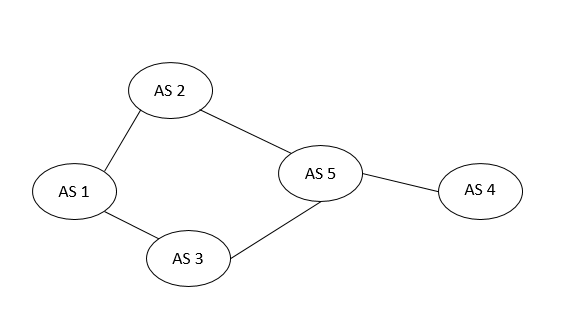
\includegraphics[width=\textwidth]{abgpexample}
  \caption{基于ASN-BGP路由示例-AS关系图}
  \label{fig:abgpexample}
\end{figure}


基于自治系统号的BGP协议域间路由的示例如下,自治系统之间的关系如图\ref{fig:abgpexample}:

\begin{itemize}
\item 自治系统4发布AS4$/$32的路由前缀,自治系统5收到自治系统4的通告,自治系统5的自治系统号可以和自治系统4的自治系统号相聚合,所以自治系统5 将收到的路由信息进行聚合。
\item 自治系统5发布聚合后的AS4$/$31和详细路由AS4$/$32,自治系统2和自治系统3收到来自自治系统5的通告。
\item 自治系统2和3分别发布聚合后的AS4$/$31和详细路由AS4$/$32,自治系统1分别收到来自自治系统2和3的通告,共4条。

\begin{table}[h]
    \centering
    \caption{自治系统收到的路由信息}
    \label{tab:oneroutinginfo}
        \begin{tabular}{|c|c|c|c|}
        \hline
            路由信息编号 & AS前缀 & 下一跳 & AS路径\\ \hline
            路由信息1 & AS4$/$32 & 自治系统2 & 2,5,4\\ \hline
            路由信息2 & AS4$/$32 & 自治系统3 & 3,5,4\\ \hline
            路由信息3 & AS4$/$31 & 自治系统2 & 2,5\\ \hline
            路由信息4 & AS4$/$31 & 自治系统3 & 3,5\\
        \hline
        \end{tabular}
\end{table}
    如上图\ref{tab:oneroutinginfo},基于AS的路由聚合算法,选择前缀更短的路由,则路由信息3和4可作为可选路由。如果是单路径机制,选择下一跳ASN 较小的路径,则路由信息3作为自治系统1的最佳路径。如果是多路径机制,最多选择两个非相交的路径,则路由信息3和4作为自治系统1的最佳路径。
    
\end{itemize}


\begin{figure}
  \centering
  % Requires \usepackage{graphicx}
  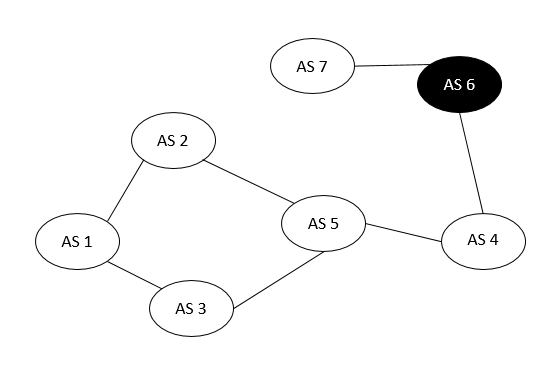
\includegraphics[width=\textwidth]{abgpexpand}
  \caption{基于ASN-BGP路由增量部署示例-AS关系图}
  \label{fig:abgpexpand}
\end{figure}

基于自治系统号的BGP协议支持现有的通告IP前缀的路由协议,因此CABA编址方式可以在网络中进行增量部署。在自治系统部署了CABA编址的情况下,如果其邻居也部署了CABA编址,则基于自治系统号的BGP协议向邻居宣告基于ASN的前缀路由信息,如果其邻居没有部署CABA编址,则基于自治系统号的BGP协议向邻居宣告原有的IP前缀路由信息。增量部署的示例如下,增量部署的自治系统之间的关系如图\ref{fig:abgpexpand}:
自治系统6没有部署CABA编址方案,其他的自治系统部署了CABA编址方案。

\section{小结}
通过了解基于AS编址的互联网可扩展路由机制框架,我们可以合理推测基于AS的编址CABA能有效减小路由表的大小和路由表的更新频率,提升路由的可扩展性。



%%% Local Variables:
%%% mode: latex
%%% TeX-master: t
%%% End:

\chapter{基于AS编址的互联网FIB表的生成与压缩情况评估}
\label{dctg}
\section{引言}
本章将详细介绍当前网络下FIB表的生成过程以及在新型编址方案CABA下采用基于ASN的BGP协议时FIB表的情况,通过对比评估新型编址环境下路由的可扩展性。
\section{数据集介绍}
实验的数据集来自Oregon大学的Route Views\onlinecite{bgpdata}工程搜集的BGP数据。进入FTP下载页面,选择13台路由器(路由器的名称为: perth, isc, linx, sydney, wide, eqix, saopaulo, nwax, telxatl, jinx, soxrs, sg, kixp),获取其2015年4月3日0点的全局路由表。

\section{当前网络下的FIB表}

\begin{enumerate}
\item 从Oregon大学的Route Views\onlinecite{bgpdata}下载13台路由器的RIB数据,下载的原始数据是二进制格式,需要工具来解析。
\item 使用libbgpdump\onlinecite{libbgpdump}解析二进制文件。需要从github上下载libbgpdump 的源代码,先执行configure,然后执行make即可生成bgpdump可执行文件,之后通过$./bgpdump -M -O outputfile inputfile$ 命令获取解析后的文件,使用M参数简化路由表项(如:TABLE\_DUMP\_V2|03/31/15 02:00:00|A|206.126.236.120|41095|0.0.0.0/0|41095 3356|IGP)。
\item 相同前缀在RIB表中可能有多条路由信息,但不考虑多路由机制,FIB表中存储的是该前缀的最优路由信息。评价最优路径有两个原则:路径的长度要最短,当路径长度相同的时候,选择下一跳自治系统号最小的路由信息。编写函数,将13台路由器的RIB表转换成FIB表。
\end{enumerate}

\section{基于AS新型编址下FIB表的设计与生成}
本章节将详细介绍基于AS新型编址下FIB表设计与生成的关键技术和增量部署的过程。
\subsection{关键技术}
将现有网络中的FIB表转换成基于AS新型编址CABA下的FIB表的主要过程如下所示:
\begin{enumerate}
\item 一个自治系统可能向外宣布多条前缀,在CABA编制下一个自治系统只需要向外宣布一条前缀。我们将当前网络中的FIB表中数据进行分析,每一项数据找到宣布这条前缀的源ASN,如果两个不同IP前缀的源ASN相同,则证明这两个不同IP前缀是由同一个自治系统宣告出来。找出同一个自治系统宣布所有前缀的表项,将其前缀替换成CABA 格式的IPv6$/$40前缀。前8位为保留位,选择IANA未使用的地址段10;之后32位为源自治系统的ASN。
\item 因为在现有网络中的FIB表中,有些前缀是由聚合的AS集合宣告的,你并不知道这些前缀究竟是由哪个自治系统向外宣告的。经过对这13台路由器的FIB 表中聚合AS集合数目大于1的表项进行统计,每个路由器约有50万条数据的FIB表中约有50条这样的表项,不足万分之一的数据。为了保证用CABA编址格式下的前缀替换原有前缀的准确性,我们舍弃这不足万分之一的聚合AS集合数目大于1的表项。
\item 替换前缀结束后,在FIB表中同一个自治系统向外公布了一条前缀,但到达这条前缀有多条路径,我们选择最优路径保留下来,其余舍弃。评价最优路径依旧遵循两个原则:路径的长度要最短,当路径长度相同的时候,选择下一跳自治系统号最小的路由信息。编写函数,将13台路由器的RIB表转换成FIB 表。
\end{enumerate}

\subsection{增量部署}
现今互联网架构和规模已经很大,协议和策略已经很完备,并且渗透到经济社会生活的方方面面,将基于AS的新型编址CABA完全部署到互联网上是不现实的,所以需要进行增量部署。本章节对两种增量部署方案的结果进行了评估,两种增量部署的方案如下:
\begin{itemize}
\item 我们得到13台路由器CABA编址下的FIB表,统计每张表的表项,表示该全局路由表中自治系统的个数。

    \begin{table}[h]
    \centering
    \caption{路由器中AS的数目}
    \label{tab:routeasnum}
        \begin{tabular}{|c|c|}
            \hline
            路由器名称 & AS数目 \\ \hline
            perth & 913 \\ \hline
            isc   & 50034 \\ \hline
            linx & 49934  \\ \hline
            kixp & 146 \\ \hline
            sydney& 50059  \\ \hline
            wide  & 49882  \\ \hline
            eqix  & 50002  \\ \hline
            saopaulo & 49953 \\ \hline
            nwax  & 49950   \\ \hline
            telxatl  & 49968 \\ \hline
            jinx  & 49685 \\ \hline
            soxrs  & 11880  \\ \hline
            sg    & 49939 \\  \hline
        \end{tabular}
    \end{table}

从上表\ref{tab:routeasnum}可以看出perth、soxrs、kixp这三台路由器可能是边界路由器,没有全局路由表的所有信息,所以我在剩余的10台路由器中随机一台路由器的FIB表,从而获取增量部署时所有的ASN,随机路由器的结果为名为saopaulo路由器。
\item 根据saopaulo路由器当前网络下的FIB表的数据,提取所有的ASN以及统计其自治系统宣布的前缀数目,每一个表项可以找到发布的前缀以及源自治系统的ASN。
\item 本章设计了三种部署方案:随机部署和根据宣告前缀数目部署。

    \begin{itemize}
        \item 随机部署:获取saopaulo路由器的当前网络下FIB表数据中前缀对应的所有ASN,随机选取所有ASN的20\%,40\%,60\%,80\%,100\%作为部署CABA编址的自治系统。
        \item 根据宣告前缀数目部署:获取saopaulo路由器的当前网络下FIB表数据中前缀对应的所有源ASN以及同一个自治系统向外宣布的前缀数目,将ASN 根据宣告前缀的数目由大到小排序,选取排序后的20\%,40\%,60\%,80\%,100\%。理论上当增量部署的程度相同时,部署宣告前缀越多的自治系统,路由表的压缩比例越多。
        \item 部署tier1层级的自治系统,tier1为互联网层级结构的最顶层,tier1层级的自治系统不论到达互联网的任何地方,都不需要支付转发和暂存等费用\cite{tier1}。
    \end{itemize}

\end{itemize}
\section{FIB表压缩情况的评估}
本章节显示FIB表的压缩结果以及对结果进行分析。
\subsection{压缩结果}
在增量部署的情况下,得到FIB表的原始数据:

\begin{table}[h]
    \centering
    \caption{随机部署:FIB压缩原始数据}
    \label{tab:origindata}
        \begin{tabular}{|c|c|c|c|c|c|c|}
            \hline
            路由器名称 & 当前网络FIB数目 & 部署20\% &部署40\% &部署60\% &部署80\% &部署100\% \\ \hline
            perth    & 8476   & 7551   & 4189   & 3360   & 3045   & 913     \\ \hline
            isc      & 573459 & 464036 & 353547 & 257451 & 170197 & 50034    \\ \hline
            linx     & 562937 & 455543 & 347739 & 253285 & 164897 & 49934     \\ \hline
            kixp     & 2329   & 2059   & 1255   & 1016   & 298    & 146        \\ \hline
            sydney   & 572895 & 462372 & 351338 & 255924 & 165075 & 50059       \\ \hline
            wide     & 558015 & 452474 & 345574 & 251150 & 165999 & 49882        \\ \hline
            eqix     & 561370 & 454054 & 347624 & 251743 & 164012 & 50002         \\ \hline
            saopaulo & 575586 & 466723 & 357205 & 258361 & 167807 & 49953          \\ \hline
            nwax     & 558075 & 451568 & 346512 & 250927 & 162610 & 49950           \\ \hline
            telxatl  & 558182 & 451432 & 346063 & 250583 & 164080 & 49968            \\ \hline
            jinx     & 536466 & 432900 & 334158 & 241083 & 157437 & 49685             \\ \hline
            soxrs    & 38037  & 32766  & 26930  & 22203  & 17930  & 11880              \\ \hline
            sg       & 557282 & 450476 & 345647 & 249168 & 162759 & 49939               \\ \hline
        \end{tabular}
\end{table}


\begin{table}[h]
    \centering
    \caption{根据宣告前缀数目部署:FIB压缩原始数据}
    \label{tab:prefixorigindata}
        \begin{tabular}{|c|c|c|c|c|c|c|}
            \hline
            路由器名称 & 当前网络FIB数目 & 部署20\% &部署40\% &部署60\% &部署80\% &部署100\% \\ \hline
            perth    & 8476   & 1977   & 1143   & 935   & 916   & 913     \\ \hline
            isc      & 573459 & 107546 & 65913  & 51985 & 50157 & 50034    \\ \hline
            linx     & 562937 & 106499 & 65513  & 5177  & 49984 & 49934     \\ \hline
            kixp     & 2329   & 306    & 208    & 181   & 160   & 146        \\ \hline
            sydney   & 572895 & 107023 & 65748  & 51974 & 50126 & 50059       \\ \hline
            wide     & 558015 & 105825 & 65335  & 51724 & 49955 & 49882        \\ \hline
            eqix     & 561370 & 106529 & 65531  & 51828 & 50049 & 50002         \\ \hline
            saopaulo & 575586 & 575586 & 65382  & 51689 & 49953 & 49953          \\ \hline
            nwax     & 558075 & 106092 & 65372  & 51745 & 49979 & 49950           \\ \hline
            telxatl  & 558182 & 106262 & 65465  & 51788 & 50013 & 49968            \\ \hline
            jinx     & 536466 & 99756  & 62580  & 51125 & 49739 & 49685             \\ \hline
            soxrs    & 38037  & 15384  & 12858  & 12003 & 11881 & 11880              \\ \hline
            sg       & 557282 & 106131 & 65447  & 51749 & 49971 & 49939               \\ \hline
        \end{tabular}
\end{table}

\begin{figure}
  \centering
  % Requires \usepackage{graphicx}
  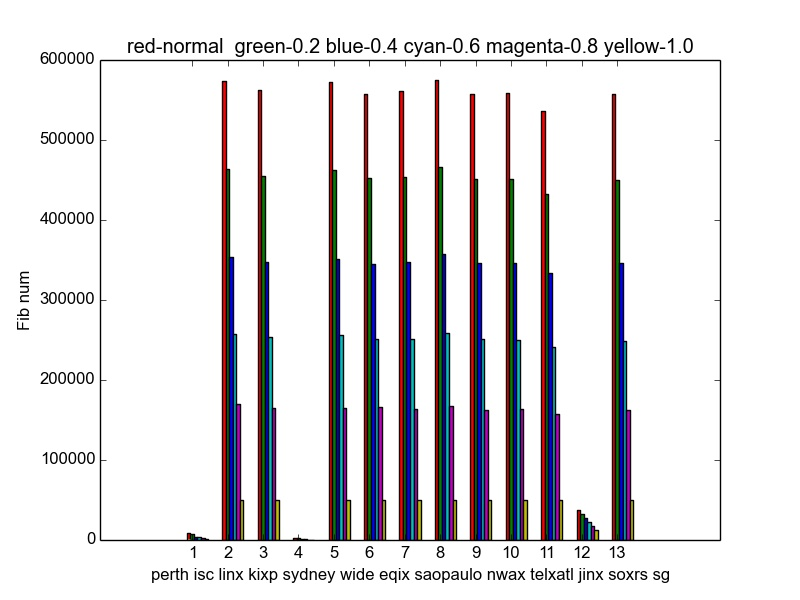
\includegraphics[width=\textwidth]{2}
  \caption{随机部署:FIB表项数目}
  \label{fig:2}
\end{figure}

\begin{figure}
  \centering
  % Requires \usepackage{graphicx}
  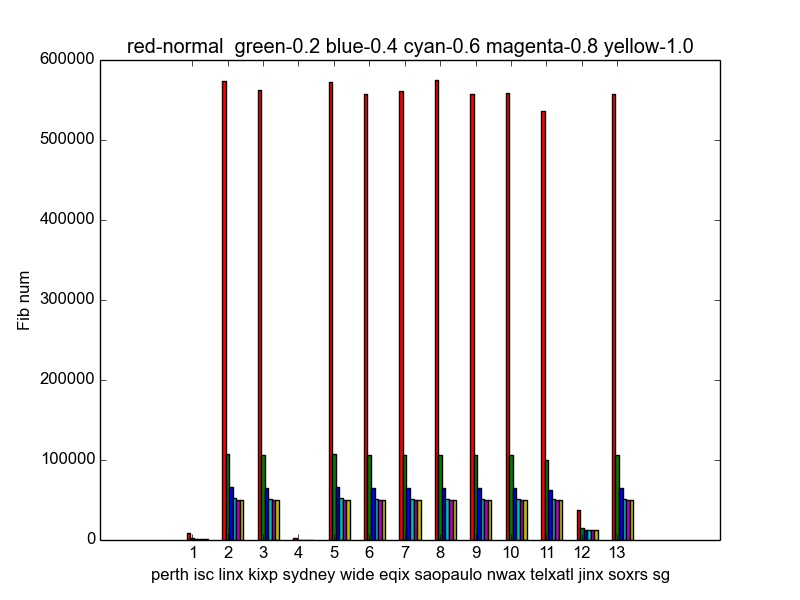
\includegraphics[width=\textwidth]{3}
  \caption{根据宣告前缀部署:FIB表项数目}
  \label{fig:3}
\end{figure}

本节我们首先看到随机部署\ref{tab:origindata}和根据宣告前缀数目部署\ref{tab:prefixorigindata}两种情况下路由表的压缩情况。从数据能很明显看到在随机部署中,FIB 表项随着部署比例的线性增加而线性减少,如图\ref{fig:2},而根据宣告前缀数目部署中FIB表项在部署比例为20\%时,大幅度减少,之后缓慢减少,如图\ref{fig:3}。说明一个自治系统向外宣告前缀越多,该自治系统采用CABA编址后,对FIB表的压缩贡献越大。由此我们可以设想,如果将Tier1的自治系统全部部署CABA编址,对FIB表的压缩程度也应该会很大,之后通过实验获得了下图的数据。

\begin{table}[h]
    \centering
    \caption{部署tier1自治系统:FIB压缩原始数据}
    \label{tab:tieronefibdata}
    \begin{tabular}{|c|c|c|c|}
    \hline
            路由器名称 & 当前网络FIB表项数目 & 部署tier1后表项数目 & 部署tier1后减少表项数目\\ \hline
            perth    & 8476   & 8476   & 0  \\ \hline
            isc      & 573459 & 562564 & 10895   \\ \hline
            linx     & 562937 & 551601  & 11336   \\ \hline
            kixp     & 2329   & 2329   & 0        \\ \hline
            sydney   & 572895 & 562573 & 10322      \\ \hline
            wide     & 558015 & 547127 &  10888         \\ \hline
            eqix     & 561370 & 551601 & 9769        \\ \hline
            saopaulo & 575586 & 564435 & 11151       \\ \hline
            nwax     & 558075 & 548597  &     9478     \\ \hline
            telxatl  & 558182 & 548524   &  9658      \\ \hline
            jinx     & 536466 & 527490    &     8976    \\ \hline
            soxrs    & 38037  & 37643      &  394   \\ \hline
            sg       & 557282 & 547893    & 9389\\ \hline
    \end{tabular}
\end{table}

\begin{table}
    \centering
    \caption{tier1自治系统号}
    \label{tab:tier1asn}
    \begin{tabular}{|c|c|c|c|c|c|}
    \hline
    174 & 209 & 286 & 701 & 1239 & 1299 \\ \hline
    2828 & 2914 & 3257 & 3320 & 3356 & 5511 \\ \hline
    6453 & 6461 & 6762 & 7018 & 12956 & - \\ \hline
    \end{tabular}
\end{table}

tier1的自治系统号来源于CAIDA官网上的数据\onlinecite{caidaasdata},下载20150201时间的AS关系数据,在其关系数据里面有tier1的ASNs见表\ref{tab:tier1asn},部署这些自治系统,我们可以看到部署17个自治系统,核心网络FIB 表的表项可以减少约1万条,约占当前网络FIB表50万表项的2\%, 验证了我们的设想。

\subsection{结果分析}
本节对三中部署方案的FIB表的压缩率进行计算绘图说明其变化趋势。

\begin{table}[h]
    \centering
    \caption{随机部署:FIB压缩率}
    \label{tab:origindatarate}
        \begin{tabular}{|c|c|c|c|c|c|c|}
            \hline
            路由器名称 & 当前网络FIB数目 & 部署20\% &部署40\% &部署60\% &部署80\% &部署100\% \\ \hline
            perth    & 8476   & 0.10913   & 0.50578  & 0.60359   & 0.64075   & 0.89228     \\ \hline
            isc      & 573459 & 0.19081 & 0.38348 & 0.55106 & 0.70321 & 0.91275    \\ \hline
            linx     & 562937 & 0.19077 & 0.38228 & 0.55007 & 0.70708 & 0.91130     \\ \hline
            kixp     & 2329   & 0.11593   & 0.46114   & 0.56376   & 0.87205    & 0.93731        \\ \hline
            sydney   & 572895 & 0.19292 & 0.38673 & 0.55328 & 0.71186 & 0.91262       \\ \hline
            wide     & 558015 & 0.18914 & 0.38071 & 0.54992 & 0.70252 & 0.91061        \\ \hline
            eqix     & 561370 & 0.19117 & 0.38076& 0.55156 & 0.70784 & 0.91093         \\ \hline
            saopaulo & 575586 & 0.18913 & 0.37941 & 0.55113 & 0.70846 & 0.91321          \\ \hline
            nwax     & 558075 & 0.19085 & 0.37909 & 0.55037 & 0.70862 & 0.91050           \\ \hline
            telxatl  & 558182 & 0.19125 & 0.38002 & 0.55107 & 0.70605 & 0.91048            \\ \hline
            jinx     & 536466 & 0.19305 & 0.37711 & 0.55061 & 0.70653 & 0.90738             \\ \hline
            soxrs    & 38037  & 0.13858  & 0.29201  & 0.41628  & 0.52862  & 0.68767            \\ \hline
            sg       & 557282 & 0.19166 & 0.37976 & 0.55289 & 0.70794 & 0.91039              \\ \hline
        \end{tabular}
\end{table}

由图\ref{tab:origindatarate}可以看出,随机部署环境下,FIB 表压缩率(FIB表减少表项\/FIB表原有表项)随着部署比例的线性增加而线性增加,明显的趋势图如\ref{fig:2rate}。

\begin{table}[h]
    \centering
    \caption{根据宣告前缀数目部署:FIB压缩率}
    \label{tab:prefixorigindatarate}
        \begin{tabular}{|c|c|c|c|c|c|c|}
            \hline
            路由器名称 & 当前网络FIB数目 & 部署20\% &部署40\% &部署60\% &部署80\% &部署100\% \\ \hline
            perth    & 8476   & 0.76675   & 0.86515   & 0.88969   & 0.89193   & 0.89228      \\ \hline
            isc      & 573459 & 0.81246 & 0.88506  & 0.90935 & 0.91254 & 0.91275    \\ \hline
            linx     & 562937 & 0.81082 & 0.88362 & 0.90803  & 0.91121 & 0.91130     \\ \hline
            kixp     & 2329   & 0.86861    & 0.91069    & 0.92228   & 0.93130   & 0.93731        \\ \hline
            sydney   & 572895 & 0.81319 & 0.88523  & 0.90928 & 0.91250 & 0.91262       \\ \hline
            wide     & 558015 & 0.81035 & 0.88292  & 0.90731 & 0.91048 & 0.91061        \\ \hline
            eqix     & 561370 & 0.81023 & 0.88327  & 0.90768 & 0.91084 & 0.91093         \\ \hline
            saopaulo & 575586 & 0.81466 & 0.88641  & 0.91020 & 0.91321 & 0.91321          \\ \hline
            nwax     & 558075 & 0.80990 & 0.88286  & 0.90728 & 0.91044 & 0.91050           \\ \hline
            telxatl  & 558182 & 0.80963 & 0.88272  & 0.90722 & 0.91040 & 0.91048            \\ \hline
            jinx     & 536466 & 0.81405  & 0.88335  & 0.90470 & 0.90728 & 0.90738             \\ \hline
            soxrs    & 38037  & 0.59555  & 0.66196  & 0.68444 & 0.68765 & 0.68767              \\ \hline
            sg       & 557282 & 0.80956 & 0.88256  & 0.90714 & 0.91033 & 0.91039               \\ \hline
        \end{tabular}
\end{table}

由图\ref{tab:prefixorigindatarate}可以看出,根据宣告前缀数目部署环境下,FIB 表压缩率(FIB表减少表项\/FIB表原有表项)在部署比例为20\%的情况下上升到很大的值,之后随着部署比例的线性增加二缓慢增加,明显的趋势图如\ref{fig:3rate}。

\begin{table}[h]
    \centering
    \caption{部署tier1自治系统:FIB率}
    \label{tab:tieronefibdatarate}
    \begin{tabular}{|c|c|c|c|}
    \hline
            路由器名称 & 当前网络FIB表项数目 & 部署tier1后FIB压缩率 & 部署tier1后减少表项数目\\ \hline
            perth    & 8476   & 0.0   & 0  \\ \hline
            isc      & 573459 & 0.01900 & 10895   \\ \hline
            linx     & 562937 & 0.01978  & 11336   \\ \hline
            kixp     & 2329   & 0.0   & 0        \\ \hline
            sydney   & 572895 & 0.01802 & 10322      \\ \hline
            wide     & 558015 & 0.01951 &  10888         \\ \hline
            eqix     & 561370 & 0.01740 & 9769        \\ \hline
            saopaulo & 575586 & 0.01937 & 11151       \\ \hline
            nwax     & 558075 & 0.01698  &     9478     \\ \hline
            telxatl  & 558182 & 0.01730  &  9658      \\ \hline
            jinx     & 536466 &   0.01673   &     8976    \\ \hline
            soxrs    & 38037  & 0.01036     &  394   \\ \hline
            sg       & 557282 & 0.01685    & 9389\\ \hline
    \end{tabular}
\end{table}

属于tier1的自治系统有17个,部署之后,对于现在的约50万的FIB表数据,可以压缩1万的表项,非常多了,占到了压缩比例的2\%,如图\ref{tab:tieronefibdatarate}但是17个自治系统相对于目前网络50000个自治系统只占0.034\%,是2\%的1\/58,也就是说部署一个tier1的自治系统相当于部署58个普通层级的自治系统。

\begin{figure}
  \centering
  % Requires \usepackage{graphicx}
  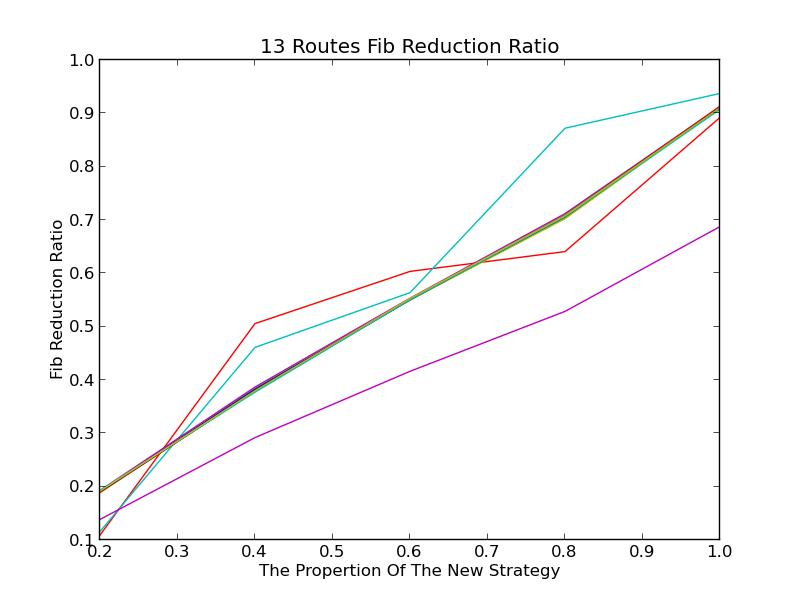
\includegraphics[width=\textwidth]{2rate}
  \caption{随机部署:FIB表项数目}
  \label{fig:2rate}
\end{figure}

\begin{figure}
  \centering
  % Requires \usepackage{graphicx}
  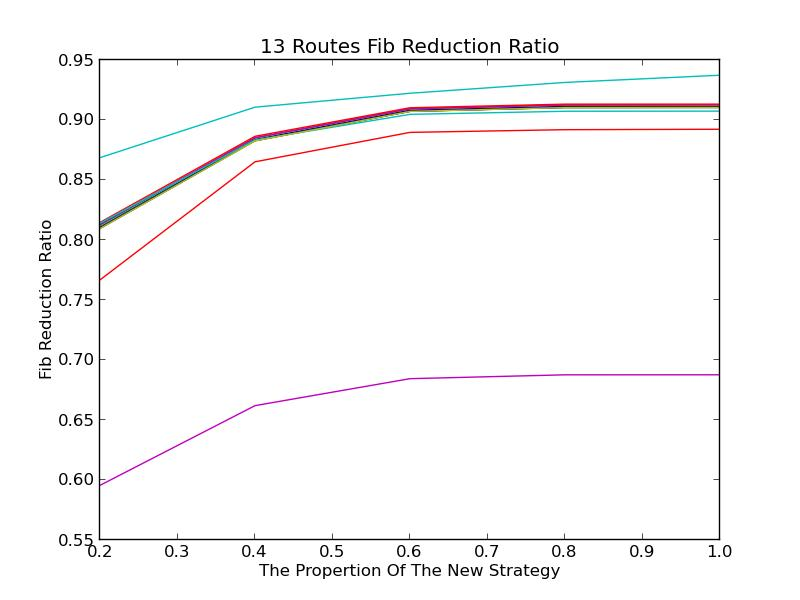
\includegraphics[width=\textwidth]{3rate}
  \caption{根据宣告前缀部署:FIB表项数目}
  \label{fig:3rate}
\end{figure}

\section{小结}
总体来看,在全部部署的情况下,FIB表的表项数目是现网络环境下FIB表表项的1\/10,增量部署的情况下,FIB表表项的压缩情况与部署自治系统向外宣布的前缀数目相关,部署自治系统向外宣告的前缀数目越多,FIB表表项的压缩情况越好。所以,我们在增量部署CABA编址时,可以考虑层级较高的自治系统和向外公布前缀较多的自治系统,这样对全局FIB的压缩作用会比较明显。


%%% Local Variables:
%%% mode: latex
%%% TeX-master: t
%%% End:

\chapter{模拟实验与性能测试}
\label{simu}
\section{引言}
前面的章节对租户网络性能的带宽保障问题进行了深入研究并提出了新的解决方案,同时设计实现了一个典型的租户应用,
为了验证所提出方案的优势,本章将对其进行实验和性能评价。

本章首先对EBG模型进行了模拟实验,之后结合DCTG系统,进行了EBG模型的性能实验。实验结果说明了,EBG模型确实
能够更加节省网络资源,同时能够解决租户需求扩张造成的问题。

\section{EBG模型性能评价实验}
\subsection{实验目的和方法}
为证明EBG模型的优势,将通过实验与其他模型进行对比,由于现有模型只有TAG能够表达应用的通信模式,所以至于TAG模型进行对比。
模拟实验将从两方面说明EBG模型的优势。

其一是从租户请求接受率上。
租户的请求并不是总能够被接受,而同样的资源,如果租户请求接受率更高,说明资源被更有效地利用了,该实验就是要
通过租户请求接受率的比较,说明EBG模型能够更好的利用数据中心资源,
从而为供应商节省成本;

其二是从租户请求扩容后,虚拟机迁移率上。
根据前面第\ref{cha:model}章的论述,租户的需求会扩展,而这会造成问题,其中主要问题就是虚拟机迁移问题。
迁移会带来严重的性能损耗,浪费大量数据中心资源,所以应当尽量避免。
这个实验通过比较迁移率,来验证EBG模型通过配置更多弹性带宽,能够有效减少迁移。

为进行模拟实验,实现了EBG模型的部署算法,并将弹性带宽为零的配置作为TAG模型(此时EBG模型等价于TAG模型)输入,进行两种模型的对比。
模拟实验在一个三层树形网络拓扑上进行,共包含2048台物理机,每个物理机包含10个虚拟机槽位。
网络上每个物理机的接入链路带宽是1Gbps,而聚合交换机和核心交换机的带宽分别为4Gbps和8Gbps。

\subsection{接受率实验}
实验中,EBG模型形如图\ref{fig:fig3.5}中的例子,因为这是最普遍的一种租户应用通信模式,
并且包含模型中的全部功能。实验随机生成大量不同组件大小,不同带宽需求的请求。
这些请求中虚拟机总数是均值为50符合指数分布的随机数,
聚合带宽保障和每台虚拟机带宽保障取不同均值的指数分布来表示不同负载的请求
(研究表明数据中心中租户虚拟机数量符合指数分布且均值为50左右,而租户的流量同样满足指数分布\cite{shieh2011sharing}),
而作为对比的TAG模型也采用均值50的指数分布随机数作为虚拟机数量,总带宽需求均值与EBG模型相同,而每台虚拟机带宽需求则是
平分总带宽需求。

实验在上一节所述网络拓扑中,生成300到500个租户请求,
通过部署算法放入网络中,计算接受的请求与总请求数的比例。
由于虚拟机槽位和网络带宽需求的限制,加上租户需求是随机生成的,
300到500个租户请求就可能将数据中心资源耗尽再也不能放入新的租户,所以实验时以连续3次部署失败作为
资源耗尽的评判标准,达成后就不再生成新的需求,而是以当前请求数来计算接受率

实验比较了不同的弹性带宽下的EBG和TAG的接受率。
$P/S$为随机生成的每虚拟机带宽保障均值与总聚合带宽保障均值的比值。
租户请求中一条边的总带宽的均值设置为1Gbps、1.5Gbps以及2Gbps。
随机生成300到500个请求后通过算法放入网络中,再计算接受率。实验结果如图\ref{fig:fig5.1}所示。

\begin{figure}[H]
  \centering
  % Requires \usepackage{graphicx}
  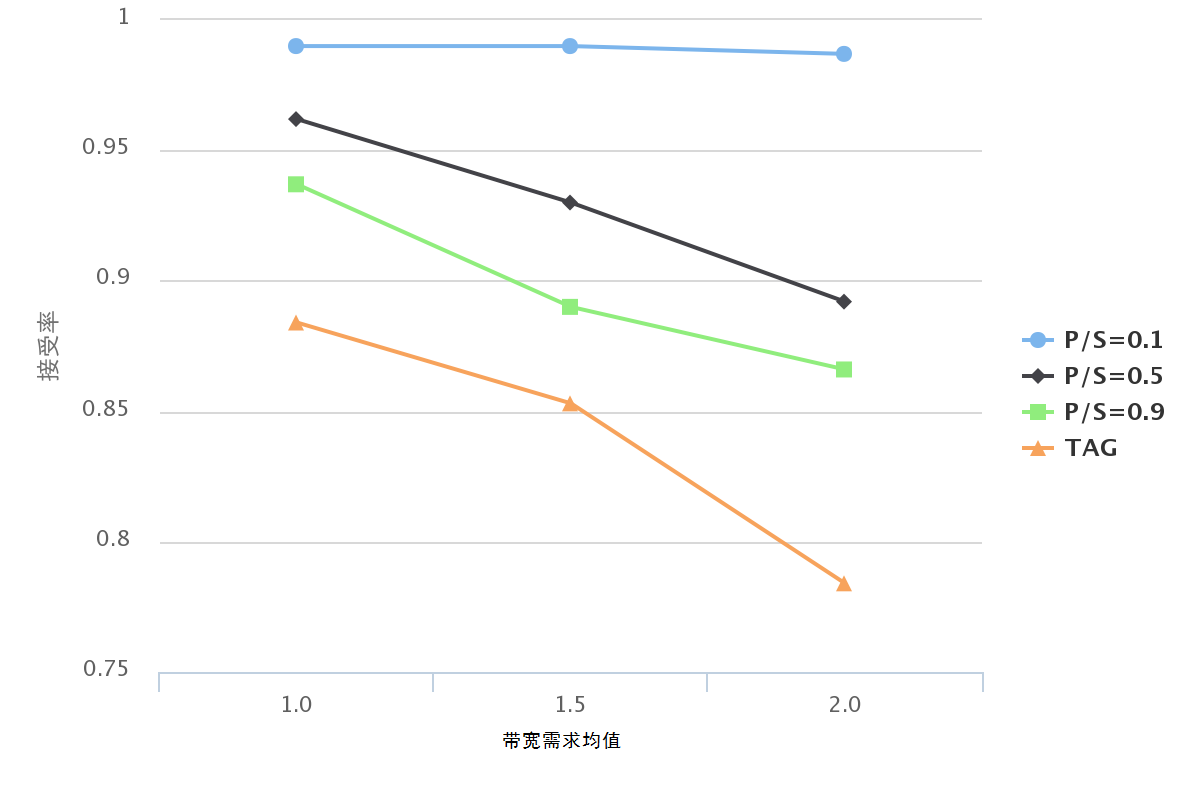
\includegraphics[width=\textwidth]{eval1}
  \caption{不同负载下EBG模型与TAG模型接受率比较}
  \label{fig:fig5.1}
\end{figure}

从图\ref{fig:fig5.1}中可以看到,随着带宽均值的提高,几种模型的接受率均有下降,
而几种模型中TAG模型的接受率最低,并且在带宽均值提高时有着明显的降低。
而EBG模型随带宽提高接受率的变化不明显,尤其当弹性带宽极高时(即$P/S$为0.1时)。
这是因为EBG模型的灵活性使得数据中心网络的资源被更有效的利用了。

\subsection{最大接受请求数实验}
另一个实验能够从侧面体现EBG的接受能力更强。实验随机生成大量请求,并进行部署,
直到连续3次分配算法失败返回,认为是数据中心网络已经接近饱和不能接受更多的租户请求,
这时比较总共接受的请求数量。这个实验目的是比较不同模型在相同的虚拟机数量和总带宽需求下,
整个数据中心网络能够接受的总请求数,能够接受更多请求的模型说明资源利用率更高。
结果如表\ref{tab:tab2}所示,其中数据是多次实验取平均值的结果,所以请求数不是整数。

\begin{table}[h]
  \centering
  \caption{不同模型最大接受请求数比较}
  \label{tab:tab2}
  \begin{tabular}{c | c c c c}
  \hline
  $P/S$ & TAG & 0.1 & 0.5 & 0.9 \\ \hline
  平均最大接受请求数 & 297.8 & 452.5 & 459.3 & 458.3 \\
  \hline
  \end{tabular}
\end{table}

从表\ref{tab:tab1}中数据可以看到,即使增加$P/S$比例,EBG能够接受的请求数量并没有受到太大影响,而由于网络拓扑中总共有20480个虚拟机槽位,每个请求的期望虚拟机数是50,所以这个最大请求数是受虚拟机槽位限制的。而TAG的接受能力却低了很多,且完全没有使用掉网络中的虚拟机槽位,可见是带宽资源限制了其接受请求。可以看到EBG模型的接受能力即使在每虚拟机带宽均值与总聚合带宽均值比值达0.9时,依然远超TAG模型,而这时不仅EBG模型请求的总带宽与TAG请求的总带宽相同,每个虚拟机的带宽保障也十分接近,EBG模型的带宽保障能力与TAG是几乎相同的。

从接受率实验中可以验证EBG模型的接受率高于TAG模型,而这正是由于弹性带宽的存在,使得EBG模型能够更好的利用数据中心的网络资源。

\subsection{租户扩容后迁移率实验}
这个实验先接受多个租户的请求,构成当前网络状态,记录下当前虚拟机的部署情况。之后随机将这些租户中的一部分的需求增加,增加其请求的虚拟机数量,之后计算旧有的虚拟机中改变位置的数量,比上虚拟机总数,得到迁移率。

实验首先在网络中部署100个虚拟机数量期望50的租户,之后按照一定比例增加虚拟机数量(在三个组件中随机选择一个),重新部署后,计算迁移的虚拟机数量与原虚拟机数量的比值。为比较TAG与EBG,租户的总带宽需求两种模型都是期望为1Gbps,而TAG的每虚拟机带宽需求按照定义由所有虚拟机平分总带宽,
结果如图\ref{fig:fig5.2}所示。

\begin{figure}[H]
  \centering
  % Requires \usepackage{graphicx}
  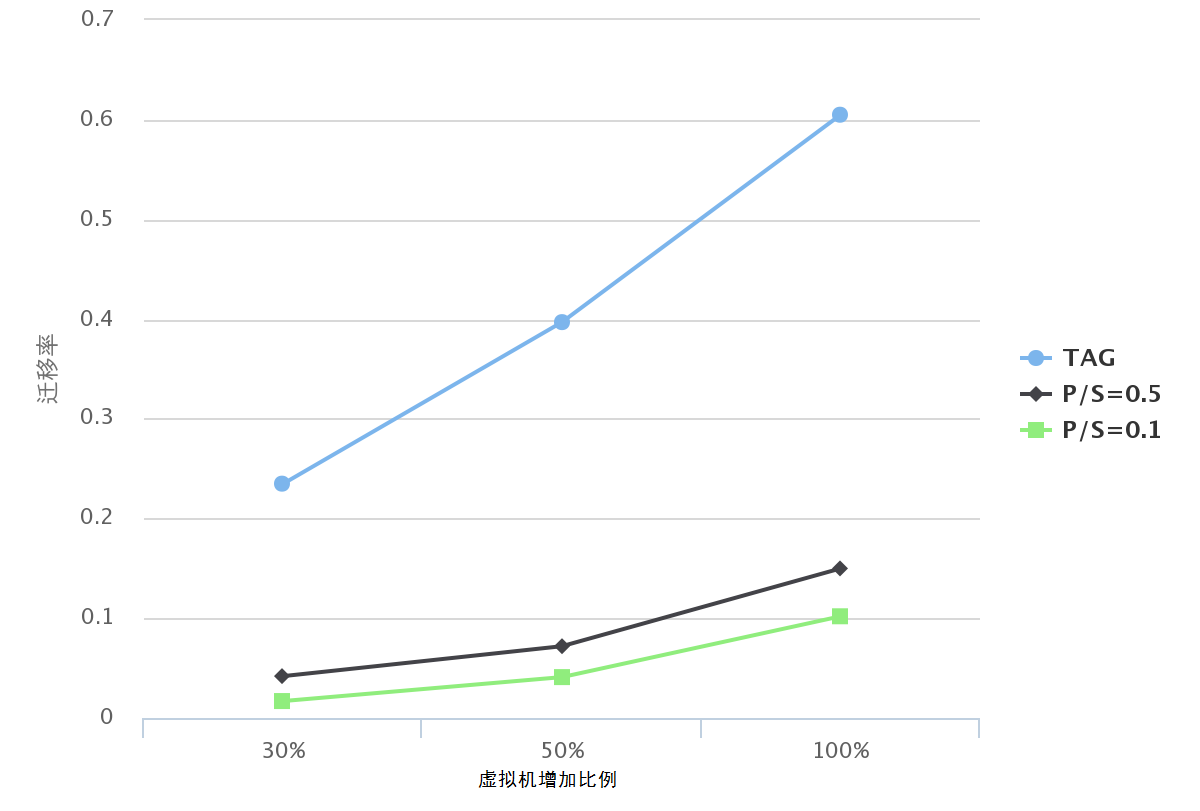
\includegraphics[width=\textwidth]{eval2}
  \caption{不同虚拟机数量增加比例下迁移率比较}
  \label{fig:fig5.2}
\end{figure}

从图中可以看到,虚拟机增加比例有30\%、50\%、100\%三种,对于EBG模型来说无论$P/S$比例是0.1还是0.5,都只有很少一部分虚拟机发生迁移。而TAG模型却有大量虚拟机迁移,在虚拟机数量增加100\% 时,甚至有60\%的原虚拟机发生迁移。

实验表明EBG模型确实能够通过充足的弹性带宽来减少发生迁移的概率,而且比起没有考虑扩容问题的TAG模型,EBG模型在这一问题上有着明显的优势。

\section{结合DCTG系统进行EBG模型性能实验}
\subsection{DCTG系统建模}
DCTG系统作为一个对网络性能十分看重的租户应用,租户带宽保障方案十分适用于这个系统。
而在各类租户带宽保障模型中,EBG模型对DCTG系统尤其适用。因为对于DCTG系统而言,只关注总带宽,而不关心每个client
的带宽,如果总带宽足够高,就能生成需要的流量,而EBG模型保障租户组件的总带宽的设计刚好符合这一点。
DCTG这样的租户应用在使用EBG模型时,能够充分享受到弹性带宽带来的优势。

要对DCTG系统使用带宽保障方案,首先需要对DCTG这一租户应用建模。使用EBG对DCTG建模如图\ref{fig:dctgmodel}。

\begin{figure}[h]
  \centering
  % Requires \usepackage{graphicx}
  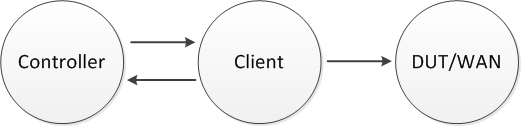
\includegraphics[scale=0.6]{DCTG}
  \caption{使用EBG对DCTG建模}
  \label{fig:dctgmodel}
\end{figure}

DCTG系统包含两个组件,controller和client,互相之间有着通信,而一般这部分的通信主要是DCTG系统的统计信息从client
汇报给controller,并不需要很大的带宽保障。另外最主要的就是从client发送出去的流量,这部分流量会发送给被测单元。
而如果DCTG测试的是云外的设备,这部分流量在云内部首先需要送到云的对外网关。所以可以看到,图中模型的最右边的组件
有可能是云内部的被测单元,也有可能是出口网关。

这个EBG模型有一个特殊之处,就是其中被测单元(或者网关)这部分并不属于租户本身,这部分并不属于租户请求,
而其在数据中心中的位置也已经确定。这样对于EBG模型的虚拟机分配算法,需要稍作改动,将这一部分看作是已经确定好位置的
组件,无需进行分配,但需要考虑其带宽保障。

\subsection{实验结果}
将DCTG建模后,就可以进行实验。实验同样对EBG模型和TAG模型,比较其接受率和迁移率。
实验中controller的组件平均大小为10VM,client的大小为平均30VM,被测单位大小平均为10VM,
随机在云中选择位置。Controller与client间的平均带宽均为500,client发送到被测单元的带宽取不同的均值来进行对比。
结果如图\ref{fig:dctgeval1}。

\begin{figure}[H]
  \centering
  % Requires \usepackage{graphicx}
  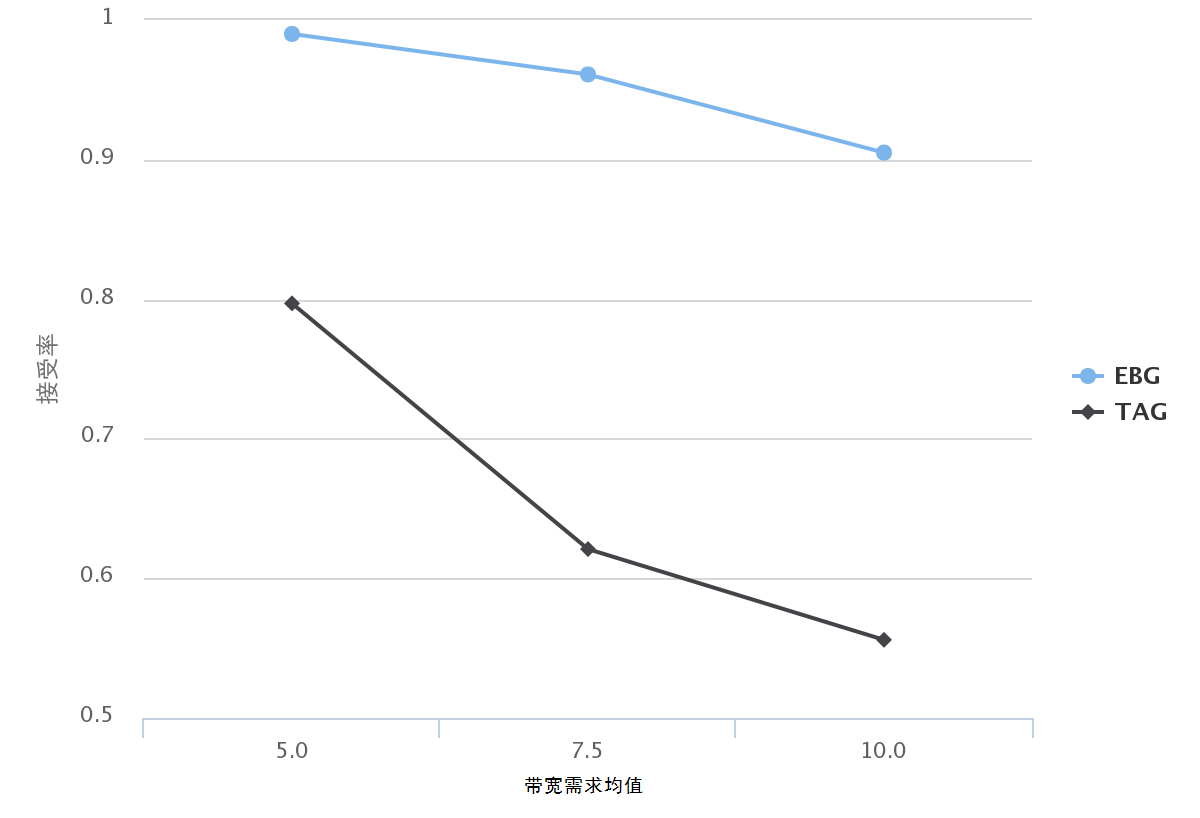
\includegraphics[width=\textwidth]{dctgeval1}
  \caption{DCTG建模的接受率比较}
  \label{fig:dctgeval1}
\end{figure}

图中可以看到,对于DCTG使用EBG和TAG分别建模,其接受率差异明显,EBG依靠弹性带宽几乎达到了100\%的接受率,
而少数不能接受的租户请求是因为被测单元的带宽限制。而TAG则接受率明显比EBG低。

\begin{figure}[H]
  \centering
  % Requires \usepackage{graphicx}
  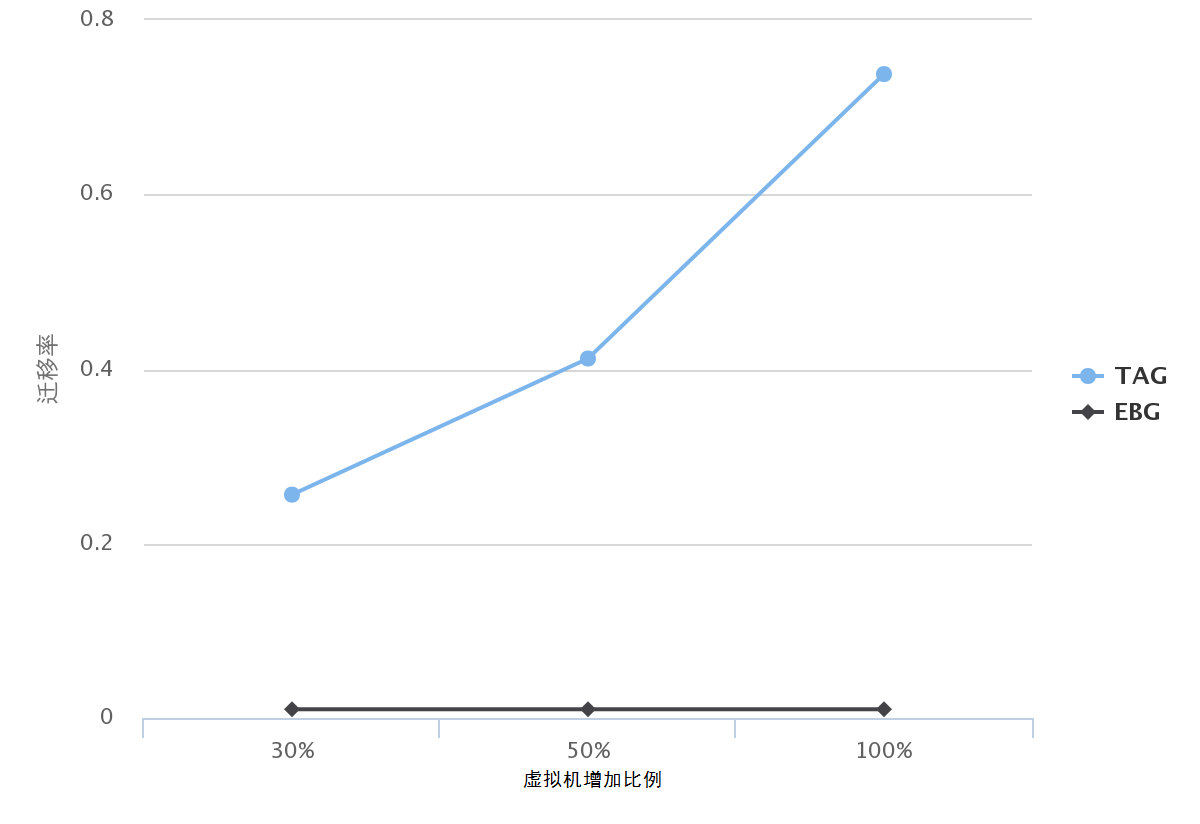
\includegraphics[width=\textwidth]{dctgeval2}
  \caption{DCTG建模的迁移率比较}
  \label{fig:dctgeval2}
\end{figure}

迁移率实验结果如图\ref{fig:dctgeval2}。EBG模型几乎不发生迁移,而TAG模型仍然发生大量迁移。
而这正是因为EBG模型建模DCTG系统,并没有每台虚拟机的带宽限制,拥有充足的弹性带宽。

由于DCTG应用的性质,使用EBG建模明显更具优势,而EBG模型的灵活性在DCTG这一类不需要每台虚拟机带宽
限制的应用上有了最大的体现。实验结果完全说明,EBG模型拥有TAG模型所不具备的灵活性,同时能够解决
租户需求变化带来的迁移问题。

\section{小结}
本章通过模拟实验,说明了EBG模型的性能优势。通过接受率的对比,说明了EBG模型能够更加有效的利用
数据中心的资源;而通过迁移率的比较,说明了EBG模型能够有效解决这一问题。同时将DCTG系统建模,进行了
实验并进一步说明了EBG模型的优势。

EBG模型的核心是弹性带宽和灵活性,通过灵活性,将租户带宽保障这一问题得以有效的解决。


%%% Local Variables:
%%% mode: latex
%%% TeX-master: t
%%% End:

\chapter{总结}
\label{conclu} 
\section{论文总结}
IaaS云服务在如今愈发重要,大量企业用户由于现有的云服务还不能提供稳定的性能而无法放心将服务器部署在
云上。提供带宽保障是让企业用户将服务器迁移到云上的重要一步,随着这项技术的发展和成熟,必然能够使得
IaaS云服务也有着更大的发展。

现在已经有了大量关于租户带宽保障的研究,然而其中缺少对于租户需求扩展这一问题的深入探讨。然而,
租户需求扩展是在使用云时必然且经常发生的情况,随着租户使用规模的扩大,这一问题发生
会十分频繁。租户需求扩展会带来虚拟机迁移的问题,而对于常见的存储类租户应用,迁移是不能接受的。
之前的租户带宽保障模型均没有能解决这一问题,所以本文提出了一种新的模型,通过巧妙的方法解决了这一问题。

本文的主要工作有:

\begin{enumerate}
\item 对租户带宽保障研究进行了综述,总结了当前已有的带宽保障方案,并介绍了当前主要的几种带宽保障模型。
\item 提出了租户需求扩展对于租户带宽保障问题产生的影响,说明了这一问题的严重性和常见性。
\item 提出了一种新的租户带宽保障模型EBG,通过模型的灵活性,既解决了迁移问题,又使新模型有了更好的性能,
能够更有效的利用云资源。并设计实现了EBG模型的部署算法。
\item 设计实现了一个典型的租户应用,基于云的测试流量生成系统DCTG。介绍了系统的设计目标,给出了详细的设计方案来
满足目标,并实现了系统进行了部署,对系统性能进行了测试说明了系统达成了设计目标。
\item 对EBG模型进行了模拟实验,通过实验说明了EBG模型的优势。同时利用EBG模型对DCTG系统进行了建模,并通过
实验进一步说明了EBG模型的优势。
\end{enumerate}

\section{未来工作展望}
未来的工作可以有几个方面,首先可以基于EBG模型实现一个真实的租户带宽保障方案,这一工作的难点主要在于
结合真实的云数据中心(比如OpenStack)来实现准入控制、虚拟机分配功能,
同时可以结合现有的work-conserving的带宽保障方案实现更加理想的租户带宽保障方案。

其次,可以进一步考察租户需求扩展对于带宽保障的影响,以及研究更好的租户需求扩展和虚拟机迁移算法,
来提高租户网络的性能。

p
%%% 其它部分
\backmatter

% 本科生要这几个索引,研究生不要。选择性留下。
\makeatletter
\ifthu@bachelor
  % 插图索引
  \listoffigures
  % 表格索引
  \listoftables
  % 公式索引
  %\listofequations
\fi
\makeatother

p
% 参考文献
% 注意至少需要引用一篇参考文献,否则下面两行可能引起编译错误。
% 如果不需要参考文献,请将下面两行删除或注释掉。
\bibliographystyle{thubib}
\bibliography{ref/refs}


% 致谢
%%% Local Variables:
%%% mode: latex
%%% TeX-master: "../main"
%%% End:

\begin{ack}
  感谢导师尹霞老师对我的指导和帮助,尹霞老师不仅在学术上,也在生活上给了我很多帮助和指导,而作为导师她也在
  平时的生活工作作风中给我们起到了榜样,同时对我遇到的各种困难和问题都给出了极大的帮助。

  感谢施新刚老师对我一直以来的辅导,施新刚老师每周抽出时间与我进行讨论,并一直在学术研究上对我进行教导,让我学会了科学的思考方式以及学术科研
  的方法。

  感谢张晗同学在研究中对我进行的帮助,张晗同学编写了十分美观方便的界面是我的系统能够使用。
  
  感谢王之梁老师、余家傲老师以及向阳、姚姜源、吴丹、耿海军、孔祥欣、田庚、王太红、郭迎亚等实验室同学们对我的帮助和照顾,
  实验室的老师同学的学术氛围也一直影响着我,使我们共同进步。
\end{ack}


% 附录
\begin{appendix}
%%% Local Variables:
%%% mode: latex
%%% TeX-master: "../main"
%%% End:

%\chapter{外文资料原文}
%\label{cha:engorg}
%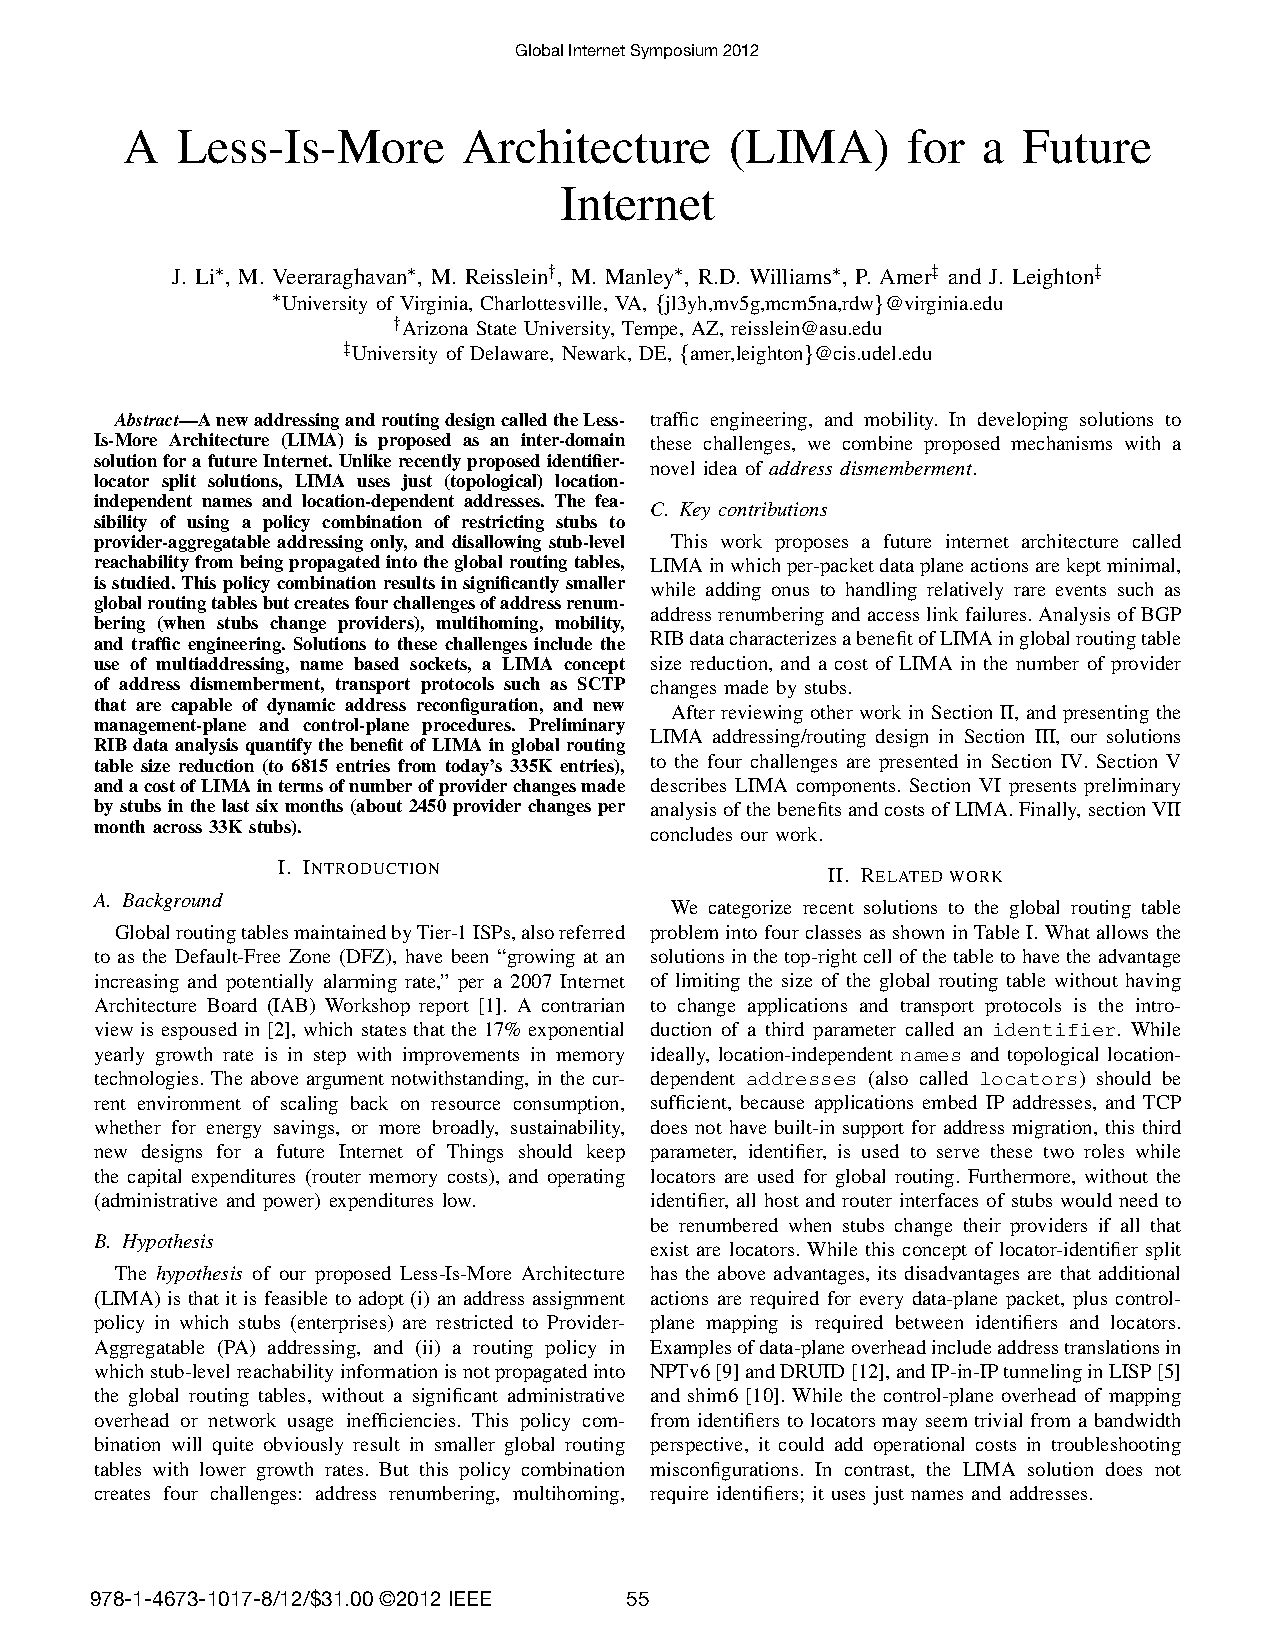
\includepdf[pages=1-6,turn=false]{ref.pdf}


\chapter{外文资料的调研阅读报告或书面翻译}

\textbf{未来互联网中的Less-Is-More结构\cite{lima}}

在未来互联网的发展中,人们提出了一种解决域间路由问题的新型寻址和路由设计,称之为Less-Is-More结构。该设计不同于最近提出的身份位置分离的解决方法,而是使用与位置无关的名称和与位置有关的地址。该设计需要结合两大相关政策,即stub必须是PA地址和stub级别的路由表信息不能扩散到全局路由表中。但政策的可行性还在研究中。该政策和设计的结合很大程度上导致全局路由表变小,但是也带来了四大挑战,即地址重编号(当stubs改变服务商),多宿主,移动性和流量工程。解决这些挑战的方法也有很多,比如使用多地址,基于端口的名字,LIMA概念的地址分解,特定传输协议(比如能够进行动态地址重配的SCTP协议),新的管理平台和控制平台程序。从基础的RIB数据分析可以确定LIMA结构可以将全局的路由表大小从现在的335K表项变成6815个表项。Stub的更新导致服务提供商的变化,维护LIMA结构的主要因素为服务提供商的改变,最近6个月平均每月有2450家服务商变化经过33k的stub。

I.	介绍\\
A.	背景\\
2007年,互联网构架委员会的一篇报告指出,全局的路由表由一级的互联网服务提供商维护,在默认的区域也同样适用的全局路由表,正在以一个逐渐增长的惊人的速率增长。与此同时,有人提出了一个相反的观点,17\%的指数年增长速率与内存技术的提高相一致。这个想法在现今为了节省能源,减少资源消耗的大趋势中,不能被接受。也就是说,在未来互联网中的设计,应该控制资本支出(路由器内存的花费)和操作支出(管理和控制)。


B.	假设\\
LIMS的假设是实行新的地址分配政策,在这个政策中,stub必须是PA地址,同时stub级别的可达信息不能传播到全局的路由表中,这不需要一个有意义的管理部门,如果传播到全局,网络使用效率将会很低。该政策很明显导致全局路由表更小,而且有更低的增长速度。但是这个政策带来了四个挑战:地址重编号,多宿主,流量工程,和移动性。解决这些挑战的方法正在发展完善中,文中的方法是将地址分解这个新颖的概念和提出的机制相结合。


C.	关键点\\
这篇论文提出名为LIMA的新型互联网结构,在这个结构中使用的数据包大小尽可能的最小,这给处理一些小概率的事件,比如地址重编号和连接链路失败,增加了负担。通过分析BGP RIB数据,我们发现LIMA结构有利于减小全局路由表的大小,而LIMA主要开销是随着stub变化服务提供商变化的数目的大小。
在浏览第二部分的相关工作之后,在第三部分描述了LIMA结构下的寻址和路由设计,第四部分解决LIMA结构带来的四个挑战,第五部分描述了LIMA的组件。第六部分对LIMA的优势和开销做了基本的分析。最后,第七部分总结了我们的工作。


II.	相关工作\\
我们把现在解决全局路由表存在问题的方法归为4类,如表1。表中右上角的方法使用了称为身份标识的第三个参数,该参数的加入使得不需要改变应用和传输协议,就可以减少全局路由表的大小。理想状况下,与位置无关的名字和与拓扑位置有关的地址足够了,因为应用中嵌套了IP地址并且TCP不支持地址迁移。当使用与拓扑位置有关的地址进行全局路由时,需要第三个参数,身份标识。如果所有存在的地址都是与拓扑位置相关的地址,一旦stub改变了自己的服务商,如果没有身份标识,所有的主机和stub 的路由接口都需要重编号。这种位置身份分离的概念有以上的优势,但也有自己的劣势。比如每个数据平台的包需要更多的空间放置额外的指令,也需要一个管理身份和位置映射控制平台。比如数据平台应该包括NPTv6和DRUID的地址翻译和在LISP和shim6中的IP-in-IP隧道。从带宽的角度看,控制平台中身份和位置的映射看起来十分琐碎,它需要增加对于错误配置的故障排除操作花费。相反,LIMA的解决方法不需要身份,只使用名称和地址。\\
LIMA的层次化寻址解决概念和平铺式寻址概念,比如ROFL,完全相反。层次化的寻址结构带来了很多问题,除了路径伸展、还有复杂管理系统、移动性和多宿主等等,都在这篇论文中有说明。

\begin{figure}
  \centering
  % Requires \usepackage{graphicx}
  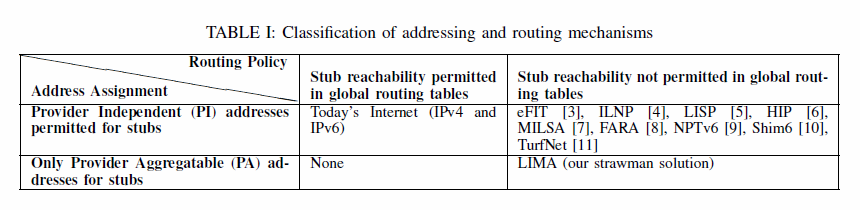
\includegraphics[width=\textwidth]{limatable1}\\
  \caption{寻址路由分类机制}\label{fig:limatable1}
\end{figure}

为什么我们的解决方案是“less-is-more”。 在第一部分B假设中提到的结合政策的LIMA和地址分解概念都能够用ipv6在网络层测试,因为ipv6支持我们设计最关键的一个需求,那就是支持多地址,我们可以通过多地址可以找到接口。LIMA是“less-is-more”,因为从现今的ipv6的解决方法角度考虑,这种方法去掉了ARP和最大长度匹配;从LISP和NPTv6的角度考虑,不需要翻译和隧道的支持;从NDN的角度考虑,NDN中的名字是基于每个包查找,NDN中使用160位地址的AIP协议,但LIMA要求更短的固定长度分解地址,比如说32位。为了避免每一包有更复杂的处理行为,LIMA对于额外的管理会做一个处罚,但仅限于地址重编号和多宿主stub中连接链路失败这两个小概率事件。暂且不论网络层,很多方面比如应用层,套接字接口,传输层协议,DHCPv6,DNS和BGP都需要做相应的变化为了支持LIMA结构,来解决该结构带来的四大问题。这些需要的变化正在当今互联网中慢慢进行。\\

III.	LIMA路由和寻址\\
LIMA主要是为了域间路由交流信息而设计的。具有额外的LIMA控制平台功能的Ipv6路由器将被使用在LIMA结构中。在该结构中,这些路由器的主要功能是作为域间路由器体现的,而不是域内路由器。在展示LIMA的寻址和路由之后,我们还讲述了两个域内stub网络的例子。\\
A.	寻址\\
简单来讲,LIMA的寻址是分层次的。这和ipv4/ipv6寻址有相似之处,需要一个全局路由前缀和一个接口身份标识,不同之处如下:

\begin{enumerate}
\item	使用自制系统号作为前缀
\item	给服务提供商分配的AS号必须是全局独一无二的AS号,而给stub分配的AS号是由它的服务提供商分配的本地服务商的AS号。这种方法不同于stub中可以在IP中使用PI地址。
\item   重新使用在域内路由网络中使用的地址作为接口身份标识,类似于ipv6地址可选选项中的MAC地址被扩展成EUI-64格式,然后被使用在interface-ID领域。
\end{enumerate}

第一个概念在参考文献第二篇中也被提及过。现今ipv4网络中前缀数目大约是335k,远大于服务提供商的AS号数目大约6185;第二个概念也在别的工作中出现过,比如eFIT,区分用户网络和服务商网络。尽管第一部分提到过,eFIT需要一个身份标识,而LIMA不需要。第三个概念和less-is-more的理念相一致,去掉了ARP和相关的安全威胁。虽然去掉了ARP,但是考虑到安全因素,我们提议在LIMA中使用DHCPv6,而不是SLAAC。MAC地址有时候是很私密的,因为它可以暴露NIC服务商的名字。如果使用动态赋值MAC地址就可以避免泄露MAC地址。为了避免欺骗,需要增加源地址过滤。


以上对LIMA寻址的描述,从IP寻址角度看,给读者提供了一个新的思路。基本的原理是把地址分成三个有区别的部分:全局独一无二的服务提供商AS号、本地服务商stub的AS号、本地stub域内地址。这三个部分对应到ipv6的地址结构上,前4个比特是全局独一无二的服务商AS号,接着4个比特是本地服务商stub的AS号,最后的8个比特是本地stub域内地址。L-DHCPv6和DNS需要进行修改来适应LIMA,L-DHPv6和L-DNS被用来标识LIMA版本的协议。一个服务商可以有多个AS号,一个服务提供商可以给它的stub分配多个AS号。


我们面临的一个问题就是如何区分一个组织是服务提供商还是stub。比如内容传送网络服务提供商:谷歌,雅虎,微软和Akamai,这些服务提供商并不能提供一条网络专线用于网路传输,现在他们的域名和很多的stub域相关联。类似的,一些客户互联网服务提供商不提供转发服务,不管是从他们的顾客来的起源和终结。我们可以通过一个给定AS的域间连接数目来区分该AS是一个服务提供商还是一个stub。这个问题在未来还可以继续研究。


B.	LIMA路由\\
LIMA路由不同于下面写的IP路由。在IP路由中,一级路由表的信息包括PI和多宿主PA stub,路由需要实现最大长度匹配。在LIMA中,一级路由表没有任何关于stub的消息,也没有最大长度匹配。相反,在LIMA中,在服务提供商网络边界路由器中的分离路由表中维护的信息是,服务商AS号和stub AS号。快速的并行查表可以通过硬件实现。当一个数据报到达目的服务商网络时,stub AS号表决定该数据报从哪个边界路由器出去。Stub边界路由器有两个表,当出口数据报经过边界路由器时,边界路由器查询服务商AS号路由表,当入口数据报进入有多个stub AS号的stub时,边界路由器查询stub AS号路由表。


C.	域内stub网络举例\\
接下来我们将通过两个域内stub的例子来说明分解寻址的概念:一个扁平化以太交换网络和一个层次结构私有ipv4路由网络。在以太网案例中,IDA就是MAC地址。我们曾经提出给L-DHCPv6服务器赋动态的MAC地址,为了强度更大的资产管理。另外,在初始化的时候,L-DHCPv6服务器要发送 { 服务提供商AS号,stub AS 号 } 对给终端。L-DHCPv6客户端在考虑地址分解的各个部分之后,在接口配置中创建他们的ipv6地址。在单个以太接口的一个多宿主stub中的一台的主机将有一个单一的IDA(MAC地址)。用MAC地址联系多对 { 服务提供商AS号, stub AS 号}产生多个ipv6地址。类似,在一个层次结构私有ipv4路由网络中的stub将会使用私有ipv4地址作为IDAs,写在ipv6地址的ID区域。


每一个主机接口对应一个权威的与IDA相关的名字。另外,一个名字对应一个主机,匹配多个接口对应的多个权威的名字。L-DNS服务器会存储所有终端名字与IDA的映射和一些简单的入口映射从组织名字映射到 { 服务提供商AS号, stub AS 号 }对。一个完全符合规定的主机域名需要结合带有主机名的组织名字。L-DNS的查询和安全动态DNS更新支持分解地址结构,可以使用stub名字或者一个特殊的终端名字。


IV.	设想的四种挑战的解决方法地址重编号


A.	地址重分配 \\

为了彻底实现全自动重新编号,LIMA采用参考资料[17],[18]的机制,该机制可以分为三类:(i)主机相关,(ii)DNS相关,(iii)路由器相关。


主机相关。关键的特征包括:(a)多地址寻址,(b)基于端口的名字(NBS)[19](c)地址分解的LIMA概念(d)SCTP[20]和MPTCP[21]的使用。多地址对带有停工的地址重编号至关重要,因为当在执行地址重编号的所有步骤中,stub能维护与旧服务提供商的连接信息1到2天。 然后,要求应用只能使用域名,避免使用NBS在应用中缓存任何地址的情况,应用对于NBS都应该是很灵活的。应用只存储或者处理名字,NBS层将名字翻译成地址。再者,地址重分配需要把新的 { 服务提供商 AS 号, stub AS 号}对广播给stub里面的所有终端,L-DHCPv6客户端收到发过来的参数,结合没有变化的IDAs生成ipv6地址,配置接口。最后,因为大部分的TCP连接都是短暂的,而且与旧服务商的连接需要每过一段时间进行维护,以防DNS缓冲查询区的数据失效,所以基于地址的一些旧的服务器不再使用后,某些连接需要终止。如果是长期的TCP连接,支持动态地址重配的传输层协议发生类似的情况,就重新连接。为了支持这个结构,我们提出使用SCTP和MPTCP。


DNS相关。接下来,让我们研究一下DNS的更新和DNS的缓存。现在的DNS服务器对每一个域名都维护一个完整的IP记录。在LIMA中,我们把数据库的每一条记录改为组织名(比如: Virginia.edu)对应一个或者多个 { 服务提供商AS号, stub AS 号 } 对,存在单个的记录匹配主机的名字和IDAs。这样的结构更容易应对服务提供商的变化。为了让缓存区DNS记录在其他stub和服务供应商中使用,stubs要维护和旧服务提供商之间的连接长达最大生存时间。

路由器相关。我们认为一个LIMA路由控制器需要运行(i)L-DHCPv6客户端,(ii)一个L-DNS客户端,(iii)拥有一个标识性的路由接口。LIMA的分解地址将采用发展比较完善的自动路由配置技术,比如Netconf。隧道配置应用应该采用名称而不是IP地址。LIMA的分解地址也需要最新的防火墙过滤技术。


B.	多宿主 \\
图一展示了在LIMA政策下,当stub收到来自每一个服务提供商的本地服务提供商stub的AS号通过其服务提供商构造的{ 服务提供商AS号, stub AS 号 } 映射对,比如A-2和B-1。如果stub和服务商A的连接断开了,考虑LIMA的路由政策的限制,一级互联网服务提供商不能到达A-2,结果没有数据包通过服务商B到达A-2。对于这个问题,我们提出了一个解决方法,那就是在stub的边界路由器和服务商A的边界路由器之间建立一条通过服务商B的隧道(图1中的点虚线),然后我们就可以把这条隧道作为stub和服务商A之间的备用链路。理论上应该规定隧道的优先级来保护经过服务商B的连通链路。在BGP中MED值可以用来设置直接连接链路作为第一选择,将备用链路作为第二选择,当链路失败时使用备用链路。


为了数据报无中断转发,有三点要求。第一,当收到路由器发来的SNMP表明直接链路连接断开的信息,为了防止使用A-2地址进行新的连接,stub的错误管理系统告诉L-DHCPv6服务器,它会发出广播信息警示所有的终端停止使用A-2全局地址。第二,错误管理系统也应该通知L-DNS服务器(LIMA版本的DNS服务器),让它不要提供A-2地址的查询结果。第三,对于正在进行的连接,终端上面的L-DHCPv6客户端应该开始SCTP或者MPTCP动态地址重配。

\begin{figure}
  \centering
  % Requires \usepackage{graphicx}
  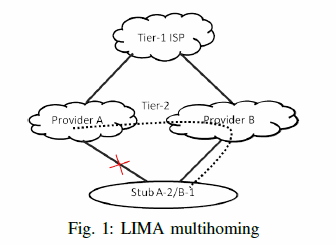
\includegraphics[width=\textwidth]{limafig1}\\
  \caption{LIMA 多宿主结构图}\label{fig:limafig1}
\end{figure}

C.	移动性\\
未来互联网设备中占据很大比例的可能是无线设备。其中,很大部分是移动,其中漫游比例可能较小。我们认为在LIMA层次化结构中,使用现今移动IP的方法来解决设备移动性的问题。


然而,为了减少路径扩展问题,我们建议结合动态DNS解决方法来增强移动IP的解决方法。现在有很多的方案提出使用安全动态DNS更新的结构来处理移动位置的管理,比如参考资料的[23],[24]。LIMA也使用了这样的方案。在LIMA中启用DNS服务器是非常有用的,因为这样当一个服务商改变的时候,stub的DNS服务器会告诉它的漫游设备,它本地发生了一些变化{ 服务提供商AS号, stub AS 号 }。在LIMA中使用移动IP可以处理DNS缓冲池中地址初始化时的连接,此外,本地stub边界路由器对它所有的终端支持本地代理,对游客支持外地代理。


D.	流量工程\\
与服务提供商相关的流量工程。在LIMA中取消现在符合ASN标准的前缀和最大前缀匹配,还有其路由政策中不允许stub的信息传到全局路由表,这些都可以导致路径延伸。比如两个主干路由器,Internet2和ESnet 。这两个路由器在洛杉矶、西雅图、芝加哥、纽约、华盛顿相互连接。ESet有两个stub客户,一个在加利福尼亚(CA),另一个在纽约(NY)。如果stub的信息可以传播出去,ESet能把它的两个stub的更长前缀匹配通知给Internet2 。从Internet2中美国堪萨斯州的路由器发给ESnet中美国加利福尼亚的包,在Internet2中将会向西朝着西雅图的路由器向前发包,如果这个包是发往美国纽约的路由器,那这个包将会往相反的方向朝着芝加哥路由器向前发包,前提条件是对于每一个路由器,在BGP更新时,都会收到来自不同路由器的信息,ESnet将会配置不同的MED值。但是,在LIMA中如果ESnet只能广播一个服务商AS号,这么有效的路由不能实现。


我们提出的解决方法是一个服务商有多个AS号,使得可以通过不同的AS号定位到这个服务商网络的不同地方。未来的工作中将会具体分析,为了实现好的交易,分配的AS号要尽可能的少,为了在低路径扩展值的情况下,不增加全局路由表的大小。


与Stub相关的流量工程。在当今的互联网中,为了平衡通过stub服务商的入口流量,一个多宿主的stub通过它的每一个服务商,有选择性地将更长前缀匹配的地址发给全局路由表。但在LIMA中,这是不可能的。我们提出了一个基于DNS和DHCP的方法来解决stub的流量工程问题。当应用程序请求选择地址的时候,stub权威的DNS服务器能整理多个地址将其返回给应用程序。对于出口流量,当告知stub的所有终端{ 服务提供商AS号, stub AS 号 }对,L-DHCPv6客户端使用不同的次序,同时用NBS层选择地址。


V.	LIMA组成部分\\
图二展示了由基于LIMA的边界ipv6路由器组成的stub网络的内部结构。使用NBS接口而不是TCP或者UDP接口修改应用。NBS为了调用套接字定义了一个新的本地类型AF\_NAME。接收方的listen和accept调用,发送方的open调用都是用域名而不是IP地址。Read和Write系统调用是NBS套接口描述器的接口函数。源地址信息放置在发送给目的地址的第一个ipv6扩展包中,接收应用会用名字而不是IP地址缓存关于源的信息(比如:颁发许可证的服务器)。


除了为了支持LIMA的分解结构而修改DHCPv6,地址重编码或者发生连接线路失败时,需要进行强制广播操作。不能使用DHCPv6重配消息,因为这个消息是用来重配一个简单的客户端的,而我们需要一类消息是stub中对所有全局地址可达终端加入或者删除{ 服务提供商AS号, stub AS 号 }对的命令。对于L\_DHCPv6服务器发送stub边界路由器接口的IDAs(也就是当今网络中的网关地址)和DNS服务器的IDA(现今DNS服务器的完整IP地址需要发给DHCP客户端)是非常高效的。因为LIMA比现在的网络更加依赖域名,预计来源于DNS客户端运行在终端上的安全动态DNS更新发生更加频繁,如图二。如果新的主机没有权威DNS更新要求的证书,L-DHCPv6服务器将会返回初始注册名字和IDA匹配。该行为要求在DHCPv6消息中增加名字。


需要对DNS进行简单地修改来适应地址分解结构。比如,原来数据库的结构应该修改成在第四部分A中提到的结构。一个自制系统地资源记录和对移动性的支持也应该加进去。
在处理链路连接失败的时候,要求LIMA错误管理系统与L-DHCPv6和L-DNS服务器通过一个协议相连接,如图2。在初始化和服务商改变的过程中,LIMA路由控制器支持路由接口的地址重分配。


为了支持LIMA的地址重分配,预计BGP也会做相应的修改。因为stub的AS号是本地服务商下的AS号,所以当BGP的更新和stub的AS号相关,stub边界路由器不仅要更新,stub的服务商边界路由器也要更新,而且服务商的AS号需要在服务商之间传播。

\begin{figure}
  \centering
  % Requires \usepackage{graphicx}
  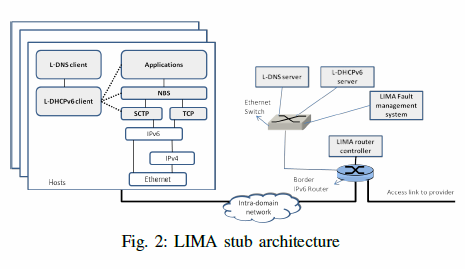
\includegraphics[width=\textwidth]{limafig2}\\
  \caption{LIMA stub结构图}\label{fig:limafig2}
\end{figure}

VI.	分析\\
评估LIMA需要几种不同的分析和原型结构,在这篇基础研究中,我们进行了两大分析。该部分A中验证使用LIMA降低全局路由表大小减少方面的优势,B中概括了地址重分配的评估。


A.	路由数据分析\\
通过分析近十年的路由器RIB数据,我们可以绘制AS总数、stub的AS数目和服务商AS数目的增长曲线,如图三。在LIMA中,全局路由表随着服务商AS的信号低速增长,现今共有6185个服务商。和335K的前缀和17\%的指数级年增长比率形成反差。

\begin{figure}
  \centering
  % Requires \usepackage{graphicx}
  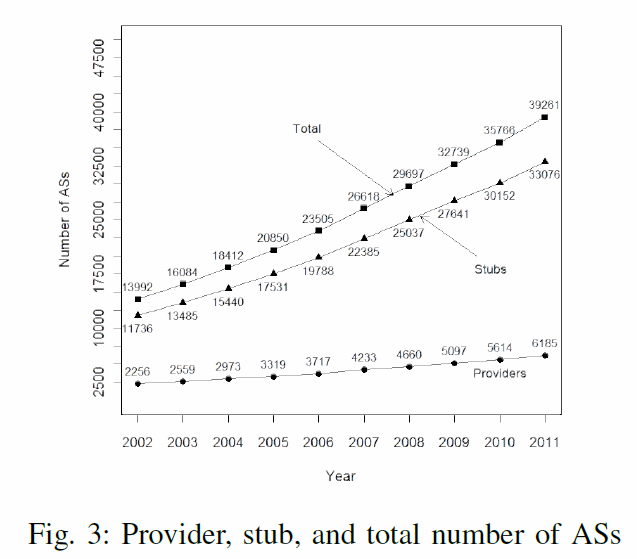
\includegraphics[width=\textwidth]{limafig3}\\
  \caption{LIMA Provider Stub AS总数}\label{fig:limafig3}
\end{figure}

B.	评估地址重编号\\
为了总结地址重分配花费代价的特征,我们分析了RIB数据为了确认stub增加或者删除服务商的频率,如表2。一些stub只增加或者减少服务商,但是增加或者减少服务商都能引起重编码操作,这两种情况都列在表2中。

\begin{figure}
  \centering
  % Requires \usepackage{graphicx}
  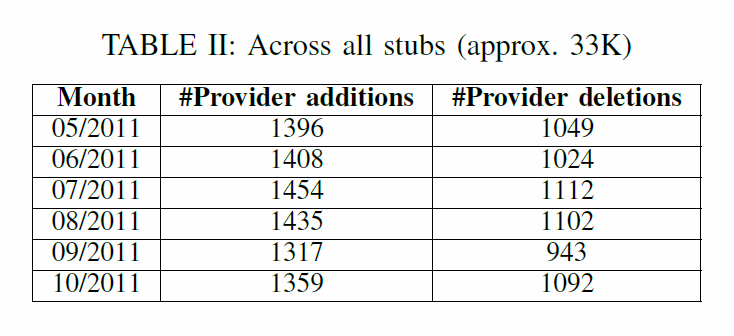
\includegraphics[width=\textwidth]{limatable2}\\
  \caption{服务商增加和减少数据}\label{fig:limatable2}
\end{figure}

图四绘制了与stub相关的每月服务商变化的平均数目,与前缀块大小的功能类似。前缀块越多,引发问题的可能性越大,即使地址重分配流程是完全自动的。随着时间的推移,总数在增长,但是比率恒定。比如,2011年和2002年,对于/24类型的stub服务商平均每月变化的数量是543和193。而2011年和2002年,stub的总数是29466和11250.因此,每个stub的服务商平均每月变化数目是2011年0.018,2002年0.017 。

\begin{figure}
  \centering
  % Requires \usepackage{graphicx}
  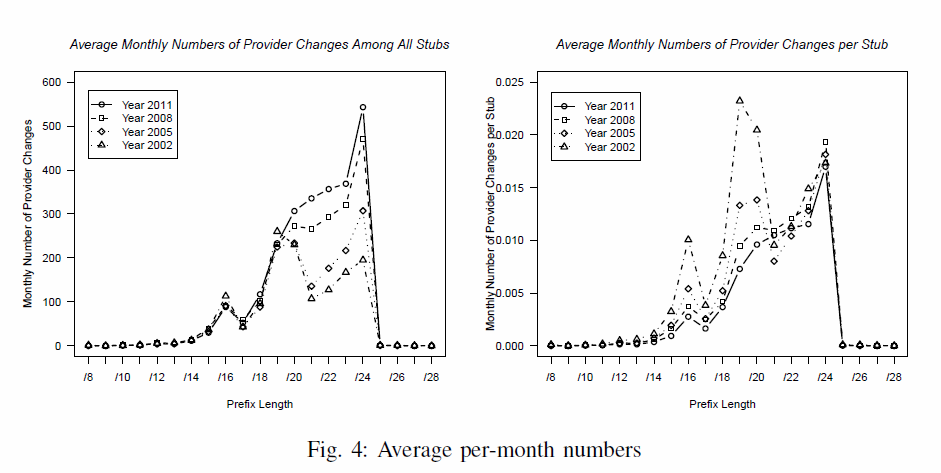
\includegraphics[width=\textwidth]{limafig4}\\
  \caption{stub相关的每月服务商变化的平均数目}\label{fig:limafig4}
\end{figure}


VII.	结论 \\
文中呈现的是一个完全地址分配和路由政策的结合,可能在今天的管理机构不流行,但是在处理地址重分配、多宿主、移动性和流量工程的问题中很灵活。相关的政策建议在stub上减少PI地址的使用,因为不允许stub级别的信息传到全局路由表中。在一个路由器比较多的stub中地址重分配在今天面临很大的挑战,需要有一些基础的改变,比如不允许在应用中使用IP地址而不是基于端口的名字,分解地址对于新的服务商AS号要做强制广播。和今天的IP相比,LIMA除了是更新的位置-身份分离方案,还按照比例缩减了每个包的指令(取消了最大长度匹配)。但是它增加了控制和管理平台,仅仅处理小概率事件,比如服务商改变和连接链路断开。LIMA 既减少了操作花费(管理和启动消耗),还通过降低内存和流程开销减少了资本支出。




%\chapter{其它附录}
%前面两个附录主要是给本科生做例子。其它附录的内容可以放到这里,当然如果你愿意,可
%以把这部分也放到独立的文件中,然后将其 \verb|\input| 到主文件中。

\end{appendix}

% 个人简历
\begin{resume}

  \resumeitem{个人简历}

  1990 年 4 月 25 日出生于 北京市。

  2008 年 9 月考入 清华大学 计算机系,2012 年 7 月本科毕业并获得 工学 学士学位。

  2012 年 9 月免试进入 清华大学 计算机系攻读 硕士学位至今。

  \resumeitem{发表的学术论文} % 发表的和录用的合在一起

  \begin{enumerate}[{[}1{]}]
  \item 一种灵活的IaaS云服务租户带宽保障模型,计算机工程与应用(已录用)
  \end{enumerate}

\end{resume}

\end{document}
